\documentclass[useAMS,usenatbib]{mn2e}
\usepackage{multirow}
\usepackage{graphicx,longtable,mathrsfs,color}
% \usepackage{txfonts}
\usepackage{csquotes}
\usepackage[usenames,dvipsnames]{xcolor} % colour
\usepackage{amssymb,amsmath,mathtools,mathrsfs} % maths
\usepackage{epsfig,subfigure,placeins,float} % plots
%\usepackage{booktabs,longtable,ctable} % tables
\usepackage{exscale,relsize} % scale 
\usepackage[normalem]{ulem} % editing
\usepackage{enumerate}
%\usepackage{dblfloatfix}
%\usepackage{fixltx2e}
\usepackage{placeins}
\usepackage{float}
%\pdfminorversion=4
\renewcommand\floatpagefraction{.9}
\renewcommand\topfraction{.9}
\renewcommand\bottomfraction{.9}
\renewcommand\textfraction{.1}   
\usepackage{placeins}
\setcounter{totalnumber}{50}
\setcounter{topnumber}{50}
\setcounter{bottomnumber}{50}
\def\com#1{{\bf {\large [#1]}}}
\setlength\textheight{652pt}
\renewcommand\floatpagefraction{.2}
\makeatletter
\def\elsartstyle{%
    \def\normalsize{\@setfontsize\normalsize\@xiipt{14.5}}
    \def\small{\@setfontsize\small\@xipt{13.6}}
    \let\footnotesize=\small
    \def\large{\@setfontsize\large\@xivpt{18}}
    \def\Large{\@setfontsize\Large\@xviipt{22}}
    \skip\@mpfootins = 18\p@ \@plus 2\p@
    \normalsize
}
\@ifundefined{square}{}{\let\Box\square}
\makeatother

\def\file#1{\texttt{#1}}
\newcommand{\hi}{H\textsc{i}}
\newcommand{\ohi}{{\Omega_\mathrm{HI}}}
\newcommand{\ob}{{\Omega_b}}
\newcommand{\om}{{\Omega_m}}
\newcommand{\be}{\begin{equation}}
\newcommand{\ee}{\end{equation}}
\newcommand{\bea}{\begin{eqnarray}}
\newcommand{\eea}{\end{eqnarray}}
\newcommand{\de}{\partial}
\newcommand{\HH}{{\cal H}}
\newcommand{\UU}{{\cal U}}
\newcommand{\DD}{{\cal D}}
\newcommand{\A}{{\cal A}}
\newcommand{\Ad}{{\cal A}_\delta}
\newcommand{\At}{{\cal A}_\theta}
\newcommand{\Am}{{\cal A}_m}
\newcommand{\Bd}{{\cal B}_\delta}
\newcommand{\Bt}{{\cal B}_\theta}
\newcommand{\Bm}{{\cal B}_m}
\newcommand{\nd}{{\dot n}}
\newcommand{\g}{\gamma}
\newcommand{\R}{{}^{(3)}\!R}
\newcommand{\Rt}{{}^{(3)}\!\tilde{R}}
\newcommand{\pid}{{\dot \pi}}
\newcommand{\pij}{{\nabla_i\partial_j \pi}}
\newcommand{\dgo}{\delta g^{00}}
\newcommand{\B}{{\cal B}}
\newcommand{\C}{{\cal C}}
\newcommand{\D}{{\cal D}}
\newcommand{\M}{{\cal M}}
\newcommand{\Y}{{\cal Y}}
\newcommand{\sR}{{\cal R}}
\newcommand{\SK}{{\cal S}}
\newcommand{\F}{{\cal F}}
\newcommand{\Z}{{\cal Z}}
\newcommand{\Hu}{{\cal H}}
\usepackage[stable]{footmisc}
\def\d{\delta}
\def\tt{\Uptheta}
\def\kv{\vec k}
\def\qv{\vec q}
\def\xv{\vec x}
\def\sv{\vec s}
\def\psiv{\vec \Psi}
\def\fe{f_{\rm eff}}
\def\Mp{M_{\rm Pl}}
\def\MM{M_{*}}
\def\Mpc{\, h^{-1} \, {\rm Mpc}}
\def\Mpccube{\, h^{-3} \, {\rm Mpc}^3}
\def\Gpc{\, h^{-1} \, {\rm Gpc}}
\def\cGpc{\, h^{-3} \, {\rm Gpc}^3}
\def\kMpc{\, h \, {\rm Mpc}^{-1}}
\def\icMpc{\, h^3 \, {\rm Mpc}^{-3}}
\newcommand{\red}[1]{\textcolor{red}{#1}}
\newcommand{\blue}[1]{\textcolor{blue}{#1}}
\def\dkmu2{\delta K_{\mu \nu}\delta K^{\mu \nu}}
\def\pmu2{  \phi_{\mu \nu}\phi^{\mu \nu}}




\title[Dark energy measurements with SKA HI Galaxy Surveys]{Dark energy measurements with  SKA HI galaxy surveys}
\author[S. Yahya, M. Silva, M. Santos, P. Okouma, R. Maartens and B. Bassett ]{S. Yahya$^{1}$\footnotemark[0]\thanks{E-mail:sahbayahya@gmail.com},  M. Silva$^{2,3}$, M. Santos$^{1,2}$, P. Okouma$^{1,4,5}$,
 \newauthor  R. Maartens$^{1,6}$ and B. Bassett$^{4,5,7}$
\\
$^{1}$Physics Department, University of the Western Cape, Cape Town 7535, South Africa\\
$^{2}$CENTRA, Instituto Superior Tecnico, Technical University of Lisbon, Lisboa 104900, Portugal\\
$^{3}$Department of Physics \& Astronomy, University of California, Irvine, CA 92697, USA\\
$^{4}$African Institute for Mathematical Sciences, Muizenberg, Cape Town 7945, South Africa\\
$^{5}$Department of Mathematics \& Applied Mathematics, University of Cape Town, Cape Town 7701, South Africa\\
$^{6}$Institute of Cosmology \& Gravitation, University of Portsmouth, Portsmouth PO1 3FX, United Kingdom\\
$^{6}$South African Astronomical Observatory, Cape Town, South Africa
}

\begin{document}

\date{\today}

\pagerange{\pageref{firstpage}--\pageref{lastpage}} \pubyear{2014}

\maketitle

\label{firstpage}
%#########################################
\begin{abstract}
%#########################################
We use Fisher forecasting and semi-analytical simulations of neutral hydrogen (HI) to predict the performance of Square Kilometer Array (SKA) HI galaxy surveys in measuring dark energy parameters.
Measurements of the tangential and radial components of the Baryon Acoustic Oscillation (BAO) length scale over a range of redshifts are the basis for constraints on the dark energy equation of state, the rate of growth of structure and the curvature of the Universe. 
\end{abstract}

\begin{keywords}
cosmology : radio surveys - galaxy power spectrum - baryonic oscillations
- dark energy
\end{keywords}


%########################################
\section{Introduction}
%########################################

The acoustic oscillation scale  in the CMB temperature anisotropies is also imprinted in the galaxy correlations. This Baryonic  Acoustic Oscillation (BAO) scale encodes the angular diameter distance $D_A(z)$ (tangential BAO scale) and the Hubble parameter $H(z)$ (radial BAO scale).
One of the key science aims of the SKA is to probe dark energy via surveys of the HI galaxy distribution. These surveys will use the HI 21cm emission line (the hyperfine transition) to detect HI galaxies -- detection of the line itself directly gives the redshift of the galaxy. The huge volumes that will eventually be covered by SKA HI galaxy surveys will allow for high-precision measurement of the BAO feature in the radial and tangential directions and at different cosmological redshifts.

The expected performance of these SKA surveys in constraining dark energy was investigated by  \citep{Abdalla:2009wr}. Here we update those results, using improved modeling of the number density and bias of the HI galaxy distribution. 
%=================================
\section*{The SKA}
%================================
%===============================================================================
%\subsection{Sensitivity and noise calculations}
%===============================================================================



%\subsection{Noise calculations}

The noise associated to the flux measured by the interferometer is assumed Gaussian with a r.m.s given approximately by
\begin{equation}
S_{\rm{rms}} \approx \frac{2 k_B T_{\rm sys}}{A_{\rm eff} \sqrt{\delta\nu\, t_p}},
\end{equation}
for an array with total effective collecting area $A_{\rm eff}$, frequency resolution $\delta\nu$ and observation time per pointing $t_p$ ($k_B$ is the Boltzmann constant). Telescope sensitivities are sometimes quoted in terms of the "System Equivalent Flux Density": SEFD $\equiv 2 k_{\rm B} T_{\rm sys}/A_{\rm eff}$ or just ''A over '': $A_{\rm eff}/T_{\rm sys}$. The effective collecting $A_{\rm eff}$ is usually 70\% to 80\% of the actual array total area depending of the efficiency of the system. Note that the expression above gives the flux sensitivity per resolution beam (not to confuse with the dish primary beam or telescope field of view). The equivalent brightness temperature uncertainty is
\be
\sigma_T= \frac{S_{\rm{rms}} c^2}{2 k_B \nu^2 (\delta\theta)^2},
\ee
where $\delta\theta$ is the angular resolution of the interferometer.
The total temperature is
\begin{equation}
T_{\rm sys}=T_{\rm inst}+T_{\rm sky}
\end{equation}
with $T_{\rm sky}\approx 60 \left(300\, {\rm MHz}/\nu \right)^{2.55}$ K and $T_{\rm inst}$ the instrument temperature which is usually higher than the sky temperature above 300 MHz.

For typical instrument specifications, the single-dish noise r.m.s can be written as:
\bea
\label{rms}
&&S_{\rm{rms}} = 368\, {\rm \mu Jy}\left(\frac{T_{\rm sys}}{20\, \rm K}\right)\times\nonumber\\
&& \left(\frac{25,000\, \rm m^2}{A_{\rm eff}}\right)\left(\frac{0.01 \rm MHz}{\delta\nu}\right)^{1/2}\left(\frac{1 \rm h}{t_{\rm p}}\right)^{1/2}. 
\eea

For a given survey area ($S_{\rm area}$) we will need $S_{\rm area}/(\theta_{\rm B})^2$ pointings where $(\theta_{\rm B})^2$ is the telescope field of view with the full width at half maximum of the beam, given by (in radians)
\begin{equation}
\theta_{\rm B} \approx \frac{1.22 \lambda}{\sqrt{(A_{\rm dish})}},
\end{equation}
where $A_{\rm dish}$ is the effective area of each dish.
The time per pointing $t_p$ is then related to the total integration time $t_{\rm tot}$ through
\begin{equation}
t_p=t_{\rm tot} \frac{(\theta_{\rm B})^2}{S_{\rm area}}.
\end{equation}
This will increase the time per pointing at the lowest frequencies.
Note that in the table below, following what is in the SKA baseline document we use instead
\begin{equation}
\frac{\theta_{\rm B}}{1{\rm deg^2}} \approx \frac{\pi}{4}\left(\frac{66\lambda}{D}\right)^2.
\end{equation}
Also, the computed phased array feed (PAF) beams are assumed constant across the band instead of going as $\lambda^2$ as above so that the time per pointing is also fixed. Table \ref{tab:telescopes} summarizes the specifications for each telescope, and Table \ref{tab:surveys} summarizes the specifications for each survey (see \cite{Bull:2014rha}).

\begin{table*}
\begin{center}
{\renewcommand{\arraystretch}{1.2} \begin{tabular}{ |l|l|l|l||l||l|l|l|l||l|l}
\hline
Telescope & Band [MHz] & z & $T_\mathrm{inst} \, [\mathrm{K}]$ & N$_{\rm dish}$ & $D_\mathrm{dish} \, [\mathrm{m}]$  & A$_{\rm eff}\, [\mathrm{m^2}]$ & Beam $[\mathrm{deg}^2]$ $^1$ & SEFD [Jy] &S$_{\rm rms}$ [$\mu$Jy] $^2$\\
 \hline
ASKAP & 700 - 1800$^5$ & (0) - 1.03 & 50$^9$ & 36 & 12.0 & 3,257 & 30$^4$ & 42.4 & 4996\\
%MeerKAT & 580 - 1015 &  0.40 - 1.45 & 29 & 64 & 13.5 & 6,413 & 2.63 & 8.61 & 1015\\
MeerKAT & 900 - 1670 &  (0) - 0.58 & 20 & 64 & 13.5 & 5,955 & 1.0 & 9.27 & 1093\\
\hline
% SKA1 - Mid & 350 - 1050 & 0.35 - 3.06 & 28 & 190 & 15 & 21,824 & 2.8 & 3.54 & 590\\
%\hline
%Mid+MK & 580 - 1015 & 0.40 - 1.45 & 28.5 & 254 & -- & 28,237 & 2.15 & 2.79 &  464\\
%\hline
%SKA1-Sur & 350 - 900$^3$ & 0.58 - 3.06 & 50 & 60 & 15.0 & 8,482 & 61$^4$ & 16.28 & 1918\\
SKA1-Sur & 650 - 1670$^3$ & (0) - 1.19 & 30 & 60 & 15.0 & 8,482 & 18$^4$ & 9.77 & 1151\\
% SKA1 - Mid & 350 - 1050 & 0.35 - 3.06 & 28 & 190 & 15 & 21,824 & 2.8 & 3.54 & 417\\
 SKA1 - Mid & 950 - 1760 & (0) - 0.50 & 20 & 190 & 15 & 26,189 & 0.75 & 2.1 & 247\\
SKA1-Sur+ASKAP & 650 - 1670$^5$ & (0) - 1.19 & 30$^5$ & 96 & -- & 11,740 & 18$^4$ & 9.1 & 832\\
%Mid+MK & 580 - 1015 & 0.40 - 1.45 & 28.5 & 254 & -- & 28,237 & 2.15 & 2.79 &  328\\
SKA1-Mid+MK & 950 - 1670 & (0) - 0.50 & 20 & 254 & -- & 32,144 & 0.8 & 1.72 & 202\\

% \multirow{1}{*}{SKA2}

\hline
SKA2 & 500 - 1200$^6$ & 0.18 - 1.84 & 20 & 250 & 50$^7$ & 400,000 & 30$^8$ & 0.14 & 16\\  
\hline
\end{tabular} }
\end{center}
\label{tab:telescopes}
\vspace{-1.4em}\caption{Telescope configurations.
$^1$ This is the primary beam (FoV) calculated at the center of the band. It changes as $\lambda^2$. For the combined telescopes, the smallest beam of the two telescopes is used.
$^2$ Flux rms for a frequency interval of 0.01 MHz and 1 hour integration using eq. \ref{rms}.
$^3$ Only 500 MHz instantaneous bandwidth.
$^4$ PAF beams assumed constant across the band.
$^5$ Assuming that ASKAP PAFs will be replaced to meet the SKA1-Sur band and instrument temperature of 30K. Assuming that only band 2 will be initially deployed.
$^6$ Band only indicative - can be changed.
$^7$ These should be stations (dense aperture arrays).
$^8$ Assuming multi-beaming to obtain large field of view.}
\end{table*}

\begin{table*}
\begin{center}
{\renewcommand{\arraystretch}{1.2} \begin{tabular}{ |l|l|l|l||l||l|l|l|l||l|}
\hline
 Telescope & Band [MHz] & Beam $[\mathrm{deg}^2]$ & S$_{\rm area}$ $[\mathrm{deg}^2]$ & $t_p$ [hours] & S$_{\rm rms}$ [$\mu$Jy]$^4$\\
 \hline
% SKA1 - Mid & 350 - 1050 & 1.38$^1$ & 5,000 & 2.76$^1$ & 355$^2$\\
ASKAP$^3$ & 700 - 1800 & 30 & 5,000 & 60 & 645\\
% MeerKAT & 580 - 1015 & 1.67$^1$ & 5,000 & 3.34$^1$ & 555$^2$\\
MeerKAT & 900 - 1670 & 1.67$^1$ & 5,000 & 3.34$^1$ & 598$^2$\\
%Mid+MK & 580 - 1015 & 1.38$^1$ & 5,000 & 2.76$^1$ & 279$^2$\\
\hline
%\hline
%SKA1-Sur$^3$ & 350 - 900 & 61 & 5,000 & 122 & 174\\
SKA1-Sur$^3$ & 650 - 1670 & 18 & 5,000 & 36 & 192\\
%SKA1 - Mid & 350 - 1050 & 1.38$^1$ & 5,000 & 2.76$^1$ & 251$^2$\\
 SKA1-Mid & 950 - 1760 & 1.38$^1$ & 5,000 & 2.76$^1$ & 149$^2$\\
 SKA1-Sur+ASKAP$^3$ & 700 - 1670 & 18 & 5,000 & 36 & 139\\
% SKA1-Mid+MK & 580 - 1015 & 1.38$^1$ & 5,000 & 2.76$^1$ & 197$^2$\\
SKA1-Mid+MK & 950 - 1670 & 1.38$^1$ & 5,000 & 2.76$^1$ & 122$^2$\\

\hline
%\line
%\hline
%\multirow{1}{*}{SKA2}
% SKA2$^3$ & 500 - 1200 & 100 & 20,000 & 50 & 3.25 & 1.6 \\
SKA2$^3$ & 500 - 1200 & 30 & 30,000 & 10 & 5\\
\hline
\end{tabular} }
\end{center}
\vspace{-1.4em}\caption{Survey specifications. We assume a total observation time of 10,000 hours. The flux rms is calculated for a frequency interval of 0.01 MHz. Values were calculated at the target frequency of 1.0 GHz, except for SKA1-Sur band 1 which has an upper limit of 900 MHz.
$^1$ The beam and time per pointing ($t_p$) are assumed to change as $(\frac{1.0\, {\rm GHz}}{\nu})^2$ across the band.
$^2$ The flux rms is assumed to change as $\frac{\nu}{1.0\, {\rm GHz}}$ across the band.
$^3$ The beam, time per pointing and flux rms are assumed constant across the band.}
\label{tab:surveys}
\end{table*}


%########################################
\section{HI Galaxy Surveys}
%########################################



For HI redshift galaxy surveys, the key inputs are \citep{Abdalla:2009wr}
the r.m.s. sensitivity ($S_{\rm{rms}}$), the detection threshold ($ n_{\sigma}$), the telescope field of view and the assumed model for HI evolution.


%=======================================
\subsection{HI galaxy redshift distribution}
%=========================================



To calculate the HI galaxy number density and bias as a function of flux r.m.s, we used the S$^3$-SAX simulations\footnote{http://s-cubed.physics.ox.ac.uk/s3\_sax}. For the detection of a galaxy, we required that at least two points on the HI line are made, that is, the width of the line has to be larger than $2\times$ the assumed frequency resolution of the survey. The idea is to get some information on the typical line double peak expected from HI 
galaxies due to their rotation. This in principle will remove any galaxy that is seen \enquote{face  on}  as it will show just a narrow peak. More evolved source detection methods can be explored, to avoid spurious detections due to RFI, we will keep this simple approach for now. A signal to noise of 10 is then required for the detection of a galaxy.

Using the S$^3$-SAX database, we used the following variables and prescription to detect HI galaxies:
\begin{itemize}
\item
$z_{\rm A}$ is  the apparent redshift (including Doppler correction).
\item
Set experiment spectral resolution to $dV = 2.1(1+z_{\rm A})$ [Km/s]. This corresponds to a frequency resolution of 0.01 [MHz] which is what has been assumed for the sensitivity calculations.
\item
$w_{\rm P}$ [Km/s]  is line width between the two horns of the HI-line profile (already corrected for the galaxy inclination), we take only galaxies where $w_{\rm P}/2 > dV$.
\item
$v_{\rm HI}$ [Jy Km/s] is the velocity-integrated line flux of the HI-line, for each galaxy we get ${\rm flux} =  v_{\rm HI} /w_{\rm P}$ and we take only galaxies where ${\rm flux}>10\times S_{\rm rms}/\sqrt{(w_{\rm P}/dV)}$.
\end{itemize}

In order to be as general as possible we didn't try to match completely the $S_{\rm rms}$ used in the query to the above survey specs. Instead we are giving results for several values so that a simple interpolation can be used if we decide to change the survey specs. In particular, if we decide to use a 5$\sigma$ cut instead of a 10$\sigma$, it is just a question of looking for the $S_{\rm rms}$ that is half the survey value (see Table~ \ref{tab:surveys}). 

To obtain the bias, the detected galaxies were put in a box, for which the power spectrum of the number counts was calculated. The bias squared was then taken as the ratio of that power spectrum to the dark matter one at $k=0.2$ h/Mpc. 
The SAX-sky simulation consists in a mock observing cone with galaxies and their properties. This simulation was built to add HI and CO properties to the galaxies obtained by \cite{2007MNRAS.375....2D} using the  millennium simulation \cite{2005Natur.435..629S}.  The millennium simulation has a box size of 500 h$^{-1}$ Mpc and its galaxies are available at  64 fixed time steps from redshifts 127 to 0. In order to properly emulate the light cone, the SAX-sky simulation used only part of each box of the millennium simulation as is described in \cite{2009ApJ...703.1890O}.  Therefore, the boxes at fixed redshifts with HI properties which can be obtained from the SAX-sky simulation are considerable smaller than 500 h$^{-1}$ Mpc in the line of sight direction. 
%
%To perform this study we used boxes with different sizes from $L_\parallel=58 h^{-1}$ Mpc and $L_\perp=100 h^{-1}$ Mpc for redshift 0.06 to $L_\parallel=162 h^{-1}$ Mpc  and  $L_\perp=398 h^{-1}$ Mpc for redshift 2.07.
%This puts a problem on the bias extraction since we cannot efficiently use modes below $k\sim 0.1$ h/Mpc. For high flux r.m.s, the number of galaxies is low and the shot noise dominates up to very small $k$s. The conclusion is that for high flux/redshift values the results should be taken as only an indication, in particular for bias above $\sim 20 \mu$Jy flux r.m.s. As an example we show in Figure \ref{pk} the dimensionless HI galaxy power spectrum at $z=1$ for different sensitivities.
%Also note that  the Millenium simulation only has galaxies with masses $\gtrsim 2\times 10^{10}$ Msun and therefore
%the bias and number density for r.m.s=1 might be affected by the lack of smaller galaxies. However this should not affect the statistics for higher r.m.s values. The cosmological analysis should compare results for different fiducial values and fully marginalise over the bias and number counts.


To be able to use the simulation output at any given redshift, we use the  formula of \cite{Obreschkow:2009ha} to fit the simulated $dN/dz$ data points from S$^3$-SAX:
  \begin{equation}
\frac{{ d}N/ {d}z}{{1 \rm deg}^2}= 10^{c_1} z^{c_2} {\rm exp}\left( - c_3 z\right), 
\label{equ: dndz}
\end{equation}
where $c_i$ are free parameters. Fig.~\ref{fig:dNOverdz_fit_sax3} shows the fitted curves and the data points. The fitted parameters are given in Table~\ref{table:free_parameters}.


\begin{figure*}
\begin{center}
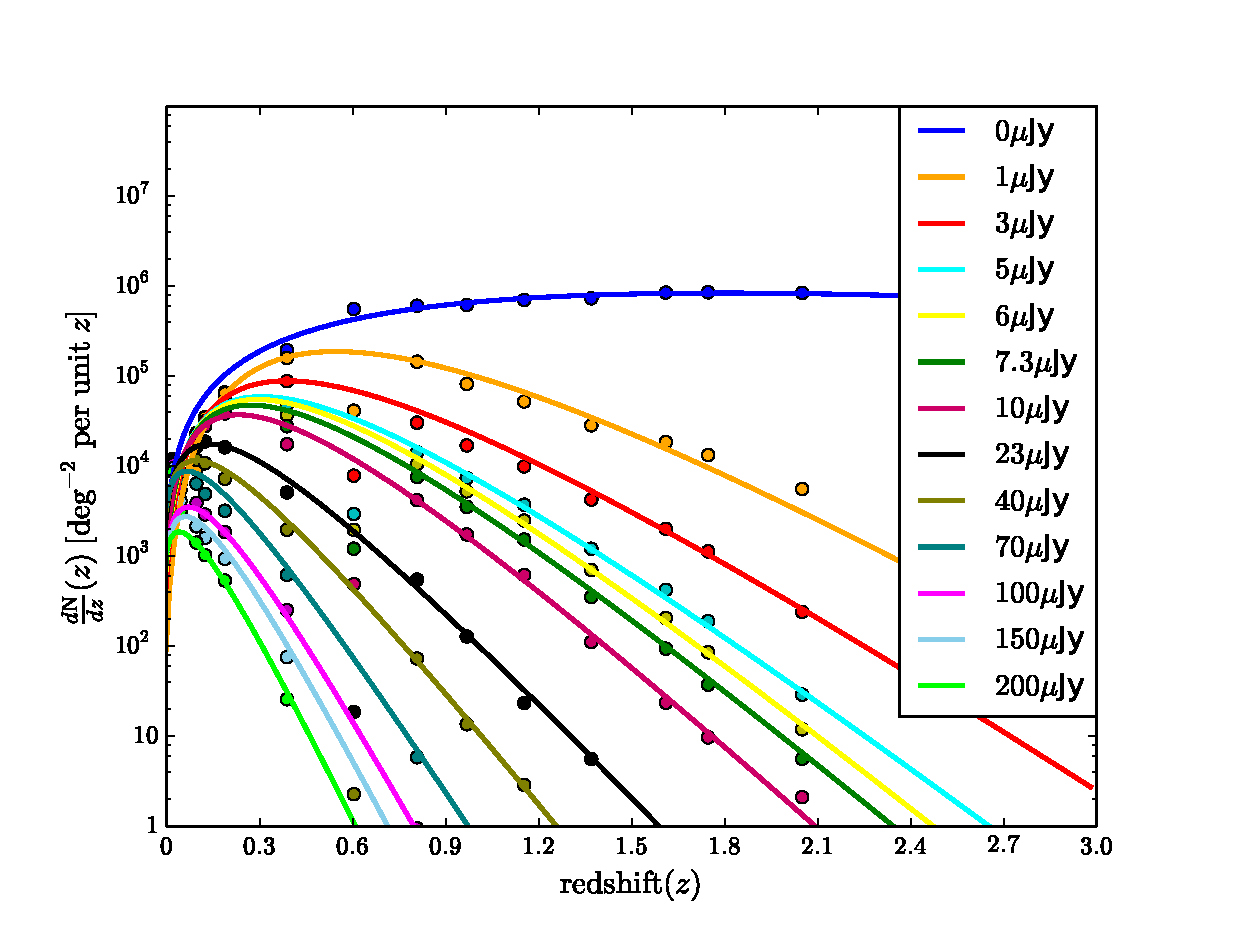
\includegraphics[width=0.8\textwidth]{plots/fittingMario_dNOverdz_using_ObreschkowFunc_diff_14bins_3.eps}
%\label{fig:bias}
%\caption{HI galaxy bias for different $S_{\rm{rms}}$.}
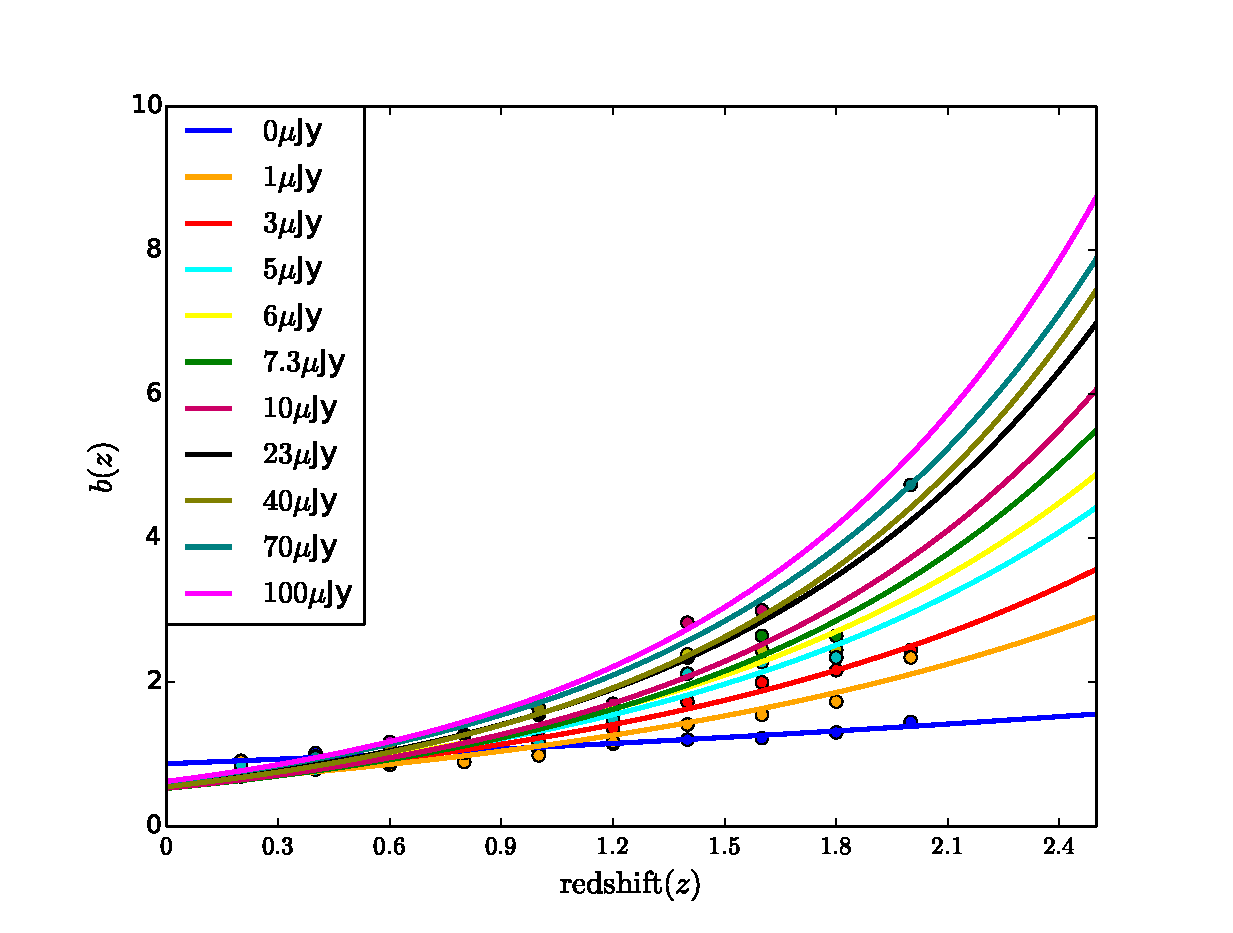
\includegraphics[width=0.8\textwidth]{plots/fitted_bias.eps}
\caption{Upper panel: Dependence of the HI galaxy redshift distribution $dN/dz$ (units: deg$^{-2}$). Note that the numbers are for different $S_{\rm{rms}}$ which will correspond to a given galaxy flux cut according to the procedure described in the text. Curves are the fits according to Eq.~(\ref{equ: dndz}) and dots are from the S$^3$-SAX simulation. Lower Panel: HI galaxy bias for different $S_{\rm{rms}}$. Note that above 70 $\mu$Jy values for high redshifts are purely extrapolations. However, this has little impact as at high z shot noise will dominate for these sensitivities.} 
\label{fig:dNOverdz_fit_sax3}
\end{center}
\end{figure*}

\begin{table}
\begin{center}
\caption{Values of the fitted parameters of Eq.~(\ref{equ: dndz}), for different $S_{\rm{rms}}$.}
\label{table:free_parameters}
\begin{tabular}{|c|c|c|c|}
\hline 
$S_{\rm rms}$ [$ \mu $Jy]& c$_1$ & c$_2$ &c$_3$      \\ 
\hline 
0 & 6.21 & 1.63 & 0.90\\
\hline
 1  & 7.33 & 3.02 &  5.34 \\
\hline
 3 & 6.91 & 2.38 &  5.84 \\
\hline
5  & 6.77 & 2.17 & 6.63 \\
\hline
 6 & 6.84 & 2.23 &  7.13 \\
\hline
7.3 & 6.76 & 2.14 &  7.36 \\
\hline
10 &  6.64 & 2.01 &  7.95 \\
\hline
23 & 6.02  & 1.43 &  9.03 \\
\hline
40 & 5.74 & 1.22 &  10.58 \\
\hline
70  &5.62 & 1.11 &  13.03 \\
\hline
100 &  5.63 & 1.41 & 15.49 \\
\hline
150  & 5.48 & 1.33 & 16.62 \\
\hline
200 & 5.00 &1.04 & 17.52 \\
\hline
\end{tabular} 
\end{center}
\end{table}
\begin{table}
\begin{center}
\caption{Values of the fitted parameters of Eq.~(\ref{bias}), for different $S_{\rm{rms}}$.}
\label{table:free_parameters_bias}
\begin{tabular}{@{}lcccc}
\hline
$S_{\rm rms}$ [$\mu$Jy ]& $c_4$& $c_5$ \\
\hline
0  & 0.8695 &    0.2338 \\
\hline
 1& 0.5863 &    0.6410 \\
\hline
3  & 0.6003 &     0.7135 \\
\hline
5  & 0.5884 &    0.8076 \\
\hline
6 & 0.5908 &  0.8455 \\
\hline
7.3 & 0.5275 & 0.9385 \\
\hline
10 & 0.5312 &     0.9745 \\
\hline
23 &0.5751 &  0.9993 \\
\hline
40 & 0.5512 &    1.0417 \\
\hline
70  & 0.6193 &    1.0179 \\
\hline
100 &0.6248 & 1.0554 \\
\hline
\end{tabular}
\end{center} 
\end{table}
\subsection{Galaxy bias from simulation}
To obtain the bias, the detected galaxies were put in a box, for which the power spectrum of the number counts was calculated. The bias squared was then taken as the ratio of that power spectrum to the dark matter one at $k=0.2$ h/Mpc. The initial box for the simulation was 500 Mpc/h, but this was further reduced along the line of sight to avoid cosmic evolution. This puts a problem on the bias extraction since we cannot efficiently use modes below $k\sim 0.1$ h/Mpc. For high flux r.m.s, the number of galaxies is low and the shot noise dominates up to very small $k$s. In the cosmic variance dominated case the error on the bias squared is just $\Delta b^2 \sim b^2/\sqrt{N}$ with the number of modes $N\sim [4 \pi k^2 \delta k]/[(2\pi)^3/{\rm V}]$, $\delta k$ is the k-bin used and V the volume of the box. The conclusion is that for high flux values the results should be taken as only an indication, in particular for bias above $S_{\rm rms} = 20 \mu$Jy. The cosmological analysis should compare results for different fiducial values and fully marginalize over the bias and number counts.
The simulated data points are shown in Fig.~\ref{fig:dNOverdz_fit_sax3} for different $S_{\rm{rms}}$ sensitivities. We use an exponential function to fit a galaxy bias $b(z)$ to the simulated data:
  \begin{equation}\label{bias}
  b = c_4 \exp({c_5z}).
  \end{equation}
Values of the fitted parameters  for each  r.m.s  sensitivity are given in Table~\ref{table:free_parameters_bias}.

%##########################################
\section{Theoretical analysis}
%##########################################


The Hubble parameter $H(z)=H_0E(z)$ and
 angular diameter distance $D_A(z)$ are given by
\begin{eqnarray}\label{EzandDz}
E&=& \sqrt{\Omega_M (1+z)^3 + \Omega_K(1+ z)^2+ 
   \Omega_{\rm de} \mathcal{F},}\\
D_{A}&=& \frac{1}{H_0\sqrt{-\Omega_K}(1+z)}\sin\left(\sqrt{-\Omega_K} \int_0^z \frac{dz'}{E(z')}\right),
\end{eqnarray}
where $\Omega_{\rm de}  = 1- \Omega_M - \Omega_K $, the dark energy is described by
\begin{equation}\label{Fz}
\mathcal{F}(z)=\exp {\int_0^z \frac{3[1+w(z')]}{1+z'}dz'} , ~~ w={p_{\rm de}\over \rho_{\rm de}},
\end{equation}
and $\Omega_M$ is the matter density ($\Omega_{{\rm cdm}} + \Omega_b$).

$H(z)$ and $D_{A}(z)$ are related directly to the comoving size of the BAO feature along and across the line of sight: 
\begin{equation}\label{DandH}
s_\Vert(z) =\frac{c \Delta z}{H(z)}\,,  \quad s_\perp(z) = (1+z) D_{A}(z) \Delta \theta.
\end{equation}
The redshift extent $\Delta z$ and angular size $\Delta \theta$ of the BAO feature are the observables. In the absence of redshift-space distortions (RSD), we have
\begin{equation}
s_\|=s_\perp=s,
\end{equation} 
where $s$ is the comoving acoustic horizon, defined at the drag epoch. Then observations determine $H$ and $D_A$ separately.
 In order to parametrize deviations from the simplest (vacuum energy) model of DE ($w=-1$), we use \citep{Chevallier:2000qy, Linder:2003nc} \begin{equation}
w(z) = w_0 + w_a \frac{z}{(1+z)}.
\label{wz}
\end{equation}

In this work, we assume a fiducial cosmological model with  cosmological parameters 
\begin{eqnarray}
&& h=0.73,~\Omega_{{\rm cdm}} = 0.24,~ \Omega_b= 0.042,~\Omega_K= 0.0, \nonumber\\ &&w_0= -1,~w_a = 0.0,~n_s=1. \label{cospar}
\end{eqnarray}

\begin{figure*}
\begin{center}
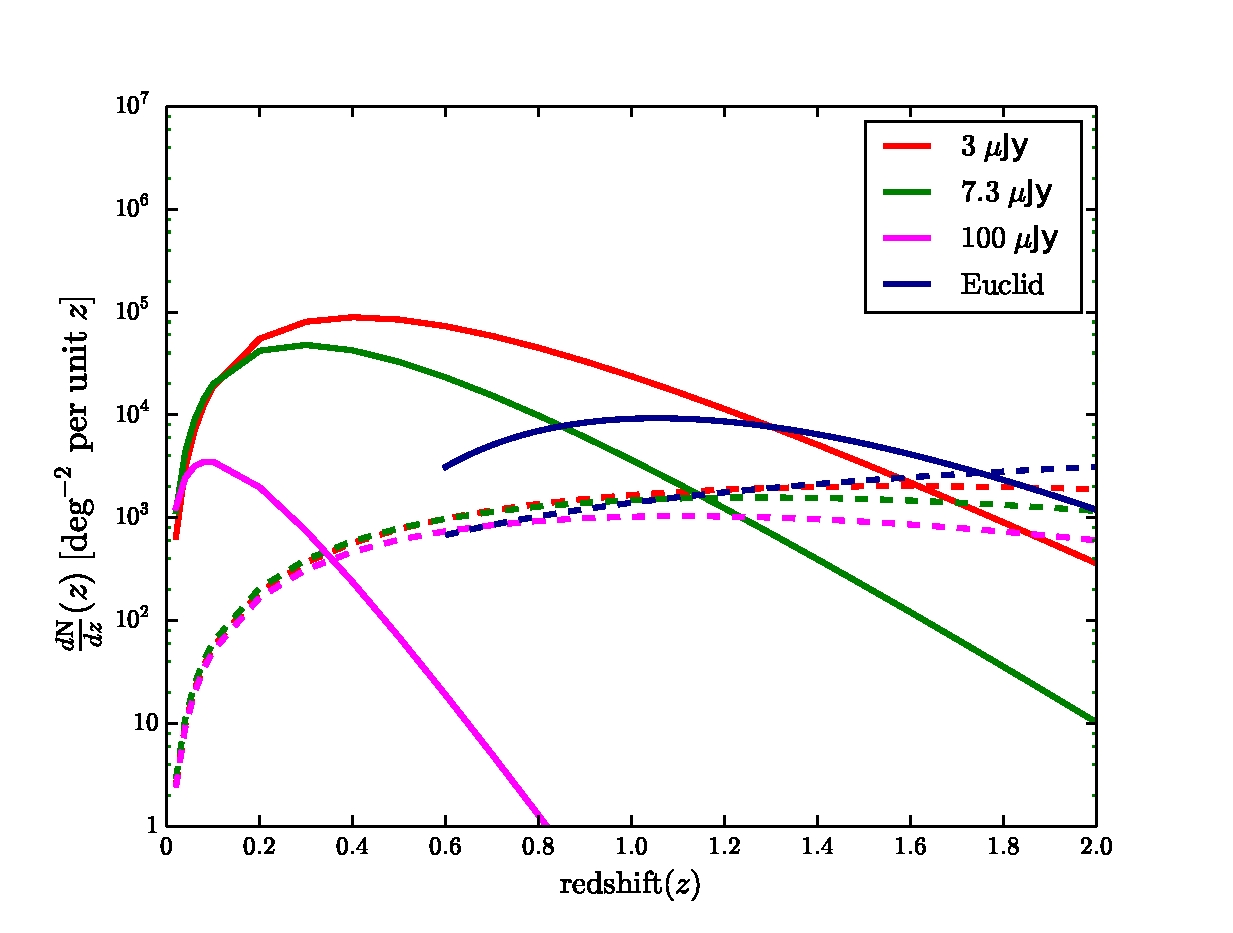
\includegraphics[width=0.8\textwidth]{plots/cosmic_Variance.eps}
\caption{Dashed lines shows the cosmic variance = shot noise for each $S_{\rm rms}$ and for Euclid redshift survey. solid lines shows $dN/dz$ for different sensitivities and for Euclid.}
\label{fig:cosmic_variance}
\end{center}
\end{figure*}


%############################################
\subsection{Forecasting method}
%##############################################

To predict the expected uncertainties in the cosmological parameters measured by the SKA, we use the Fisher forecasting method.
 The Fisher matrix is
\begin{equation}
 F_{ij} \simeq \sum_n \frac{1}{(\Delta x_n)^2}\frac{\partial
    x_n}{\partial \theta_i}\frac{\partial x_n}{\partial
  \theta_j} ,
\end{equation}
where $\theta_i$ are the cosmological parameters, $x_n$ are the data and $\Delta {x_n}$ are  the expected uncertainties on the data, which  depend on the design of the experiment.
The Fisher matrix  can be expressed in terms of the observed redshift-space power spectrum $P^z$ and the number density of galaxies $n$:
\begin{eqnarray}  
F_{ij}=
\int_{-1}^{1}d\mu \int_{k_{\rm min}}^{{k_{\rm max}}} {k^2dk\over 8\pi^2} \frac{\partial  P^z}{\partial \theta_i} \frac{\partial P^z}{\partial \theta_j}
{V_{\rm survey}\over [P^z+n^{-1}]^2}.
 \label{eq:Fij}
\end{eqnarray}

The real-space power spectrum $P$ is related to $P^z$ by
\begin{eqnarray}
P^z(k,\mu)&=& R(\mu,k)P(k),\\
R(\mu,k)& =& (1+\beta\mu^2)^2\exp{\left(-k^2\mu^2\Sigma_z^2 \right)}.\label{eq:Rsig}
\end{eqnarray}
Here $\mu=\vec{k}\cdot\vec{e}/k$, and $\vec{e}$ is the line-of-sight direction. 
The linear RSD parameter $\beta$ is given in terms of the growth rate $f$ by \citep{Komatsu:2008hk}
\begin{equation}
     \beta(z)=\frac{f(z)}{ b(z)},~~~f(z)=-{d\ln D(z) \over d\ln (1+z)},
\end{equation}
where $D$ is the growing mode of matter perturbations, normalized so that $D\to (1+z)^{-1}$ at high $z$.
Nonlinear RSD are modelled by the exponential damping term, where
\begin{equation}
\Sigma_z= \frac{\sigma_z (1 +z)}{H(z)},
\end{equation}
and $\sigma_z$ is the error on redshift. The survey volume is given by

\begin{equation}\label{Vsurvey}
V_{\rm survey} = \left(\frac{\pi}{180}\right)^2 \ S_{area}\int^{z_{\rm min}}_{z_{\rm max}} \frac{dV}{dz}, 
\end{equation}
where $dV/dz$  is differential comoving volume per unit area, in units of $h^{-3} \ {\rm Mpc}^3$ \citep{Hogg:1999ad}.
\begin{center}
\begin{figure}
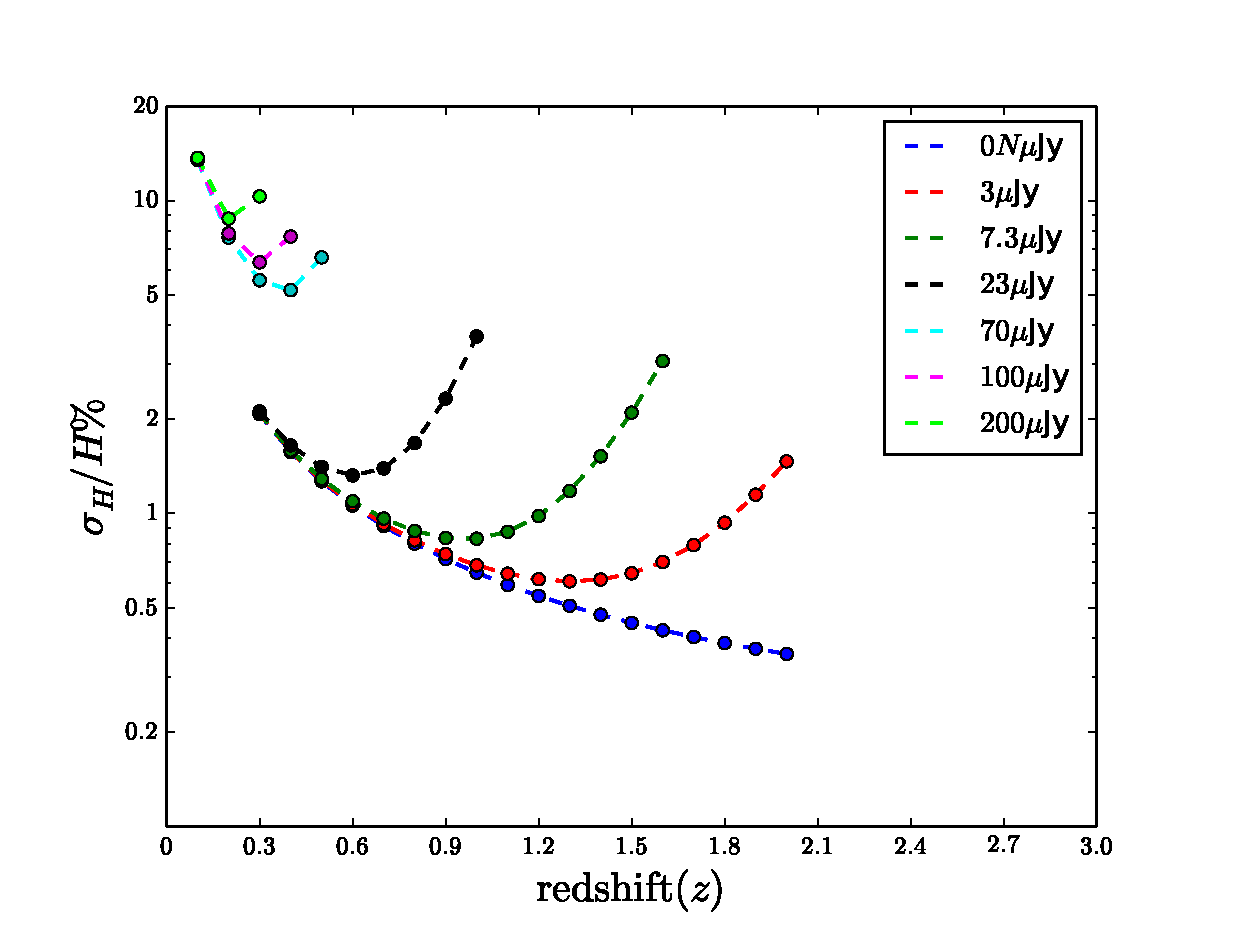
\includegraphics[height=7cm,width=9cm]{plots/output_lnH_mario_bias.eps}
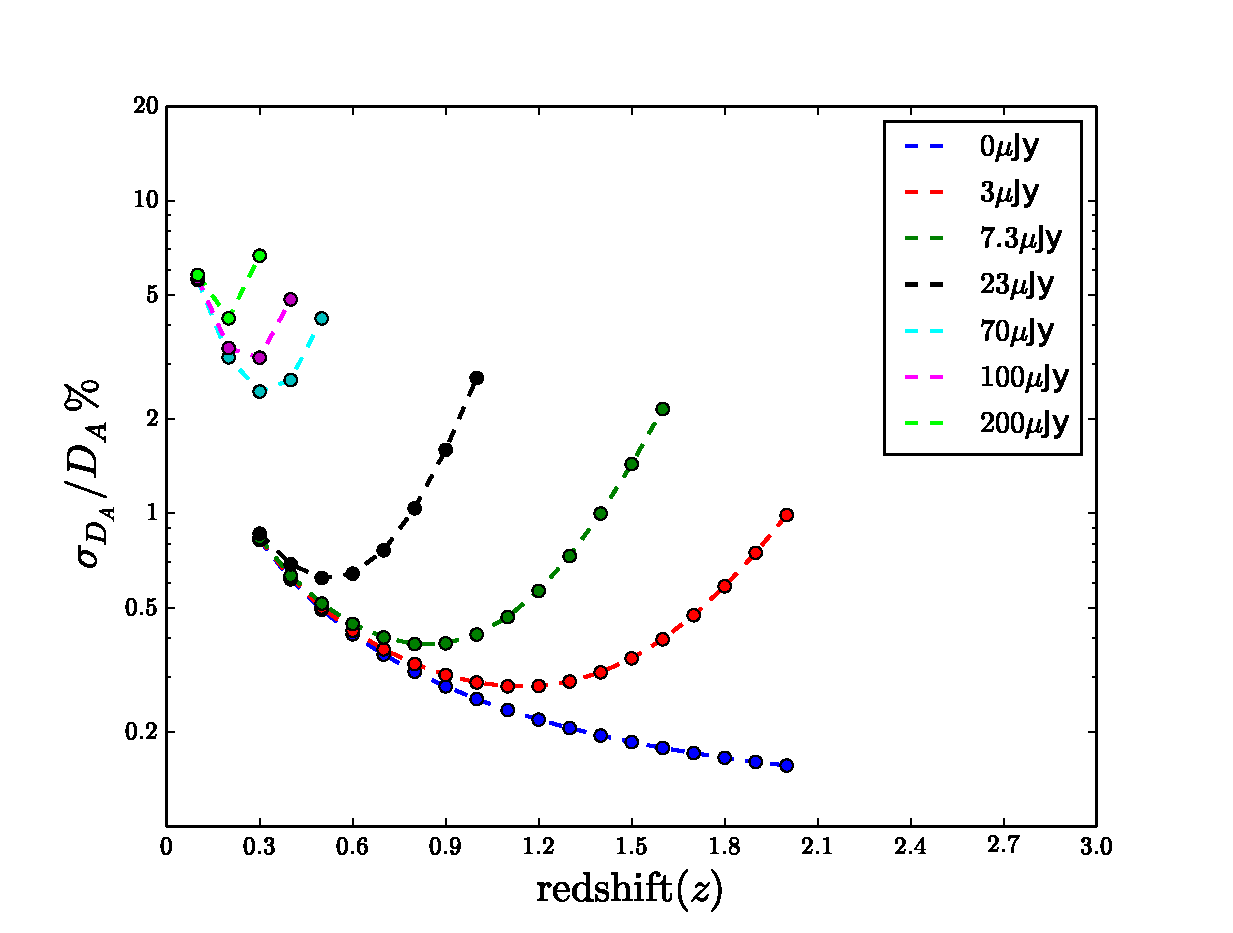
\includegraphics[height=7cm,width=9cm]{plots/output_lnda_mario_bias.eps}
\includegraphics[height=7cm,width=9cm]{plots/output_beta_mario_bias.eps}
\caption{Top: fractional error ($\%$)  on  the radial component ($\sigma_H/H \%$) . Middle:  fractional error ($\%$) on the tangential component  ($\sigma_{D_A}/D_A  \%$). Bottom: the fractional error ($\%$) on $\beta$ ($\sigma_\beta/\beta \%$).}
\label{fig:fraction}
\end{figure}
\end{center}

\begin{center}
\begin{figure}
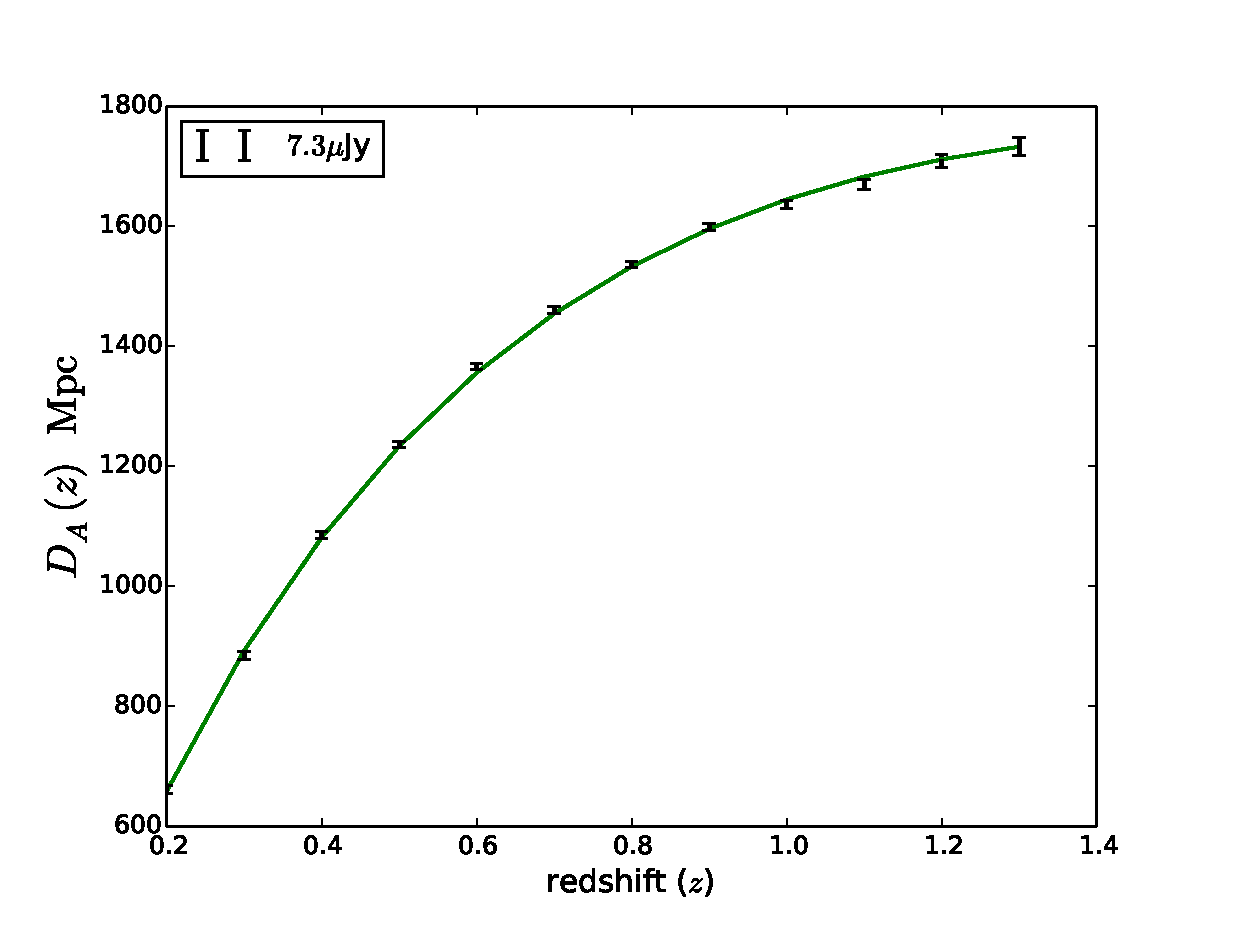
\includegraphics[height=7cm,width=9cm]{plots/DA_errs_7point3mJy_modified_diff_14bins.eps}
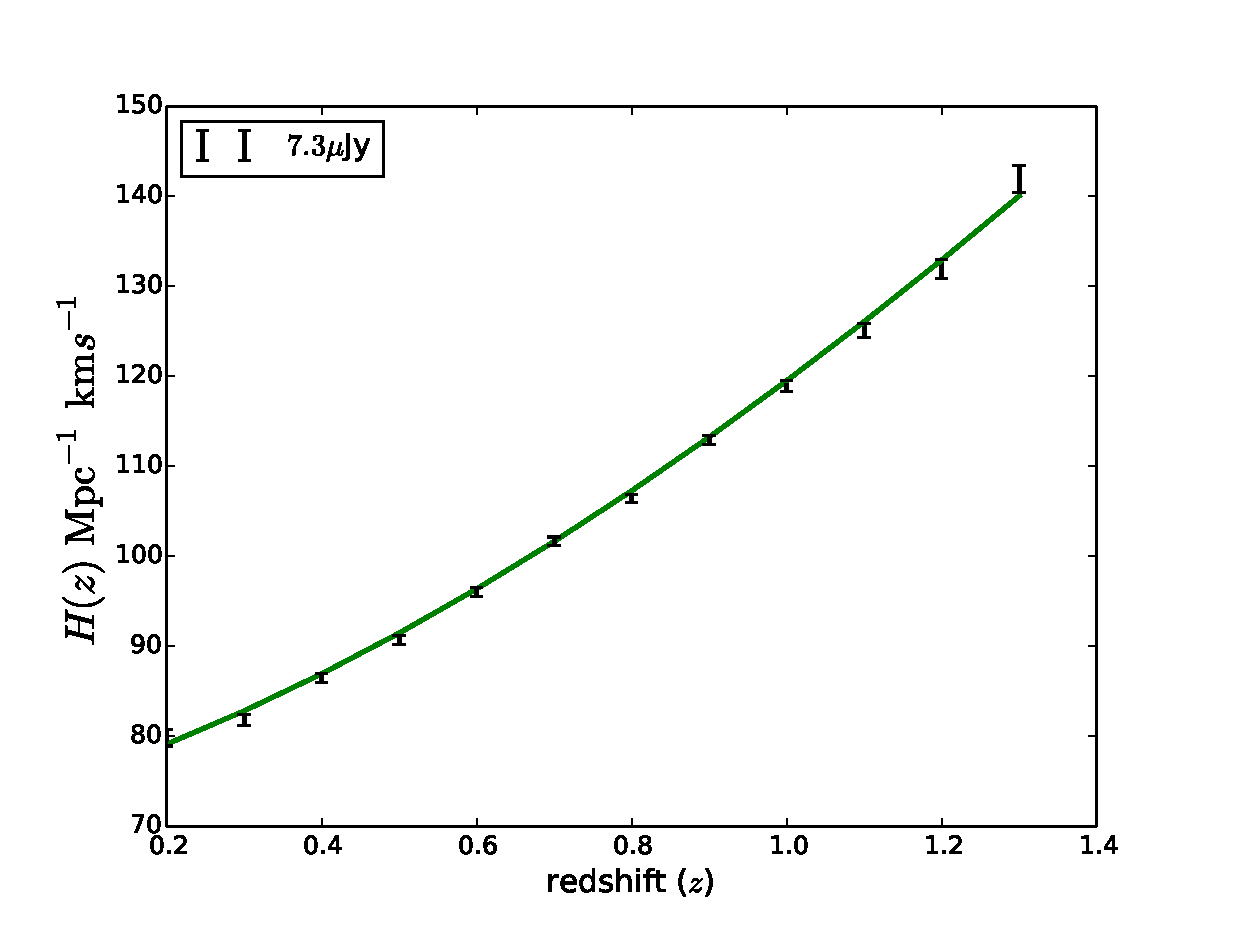
\includegraphics[height=7cm,width=9cm]{plots/Hz_errs_7point3mJy_modified_diff_14bins.eps}
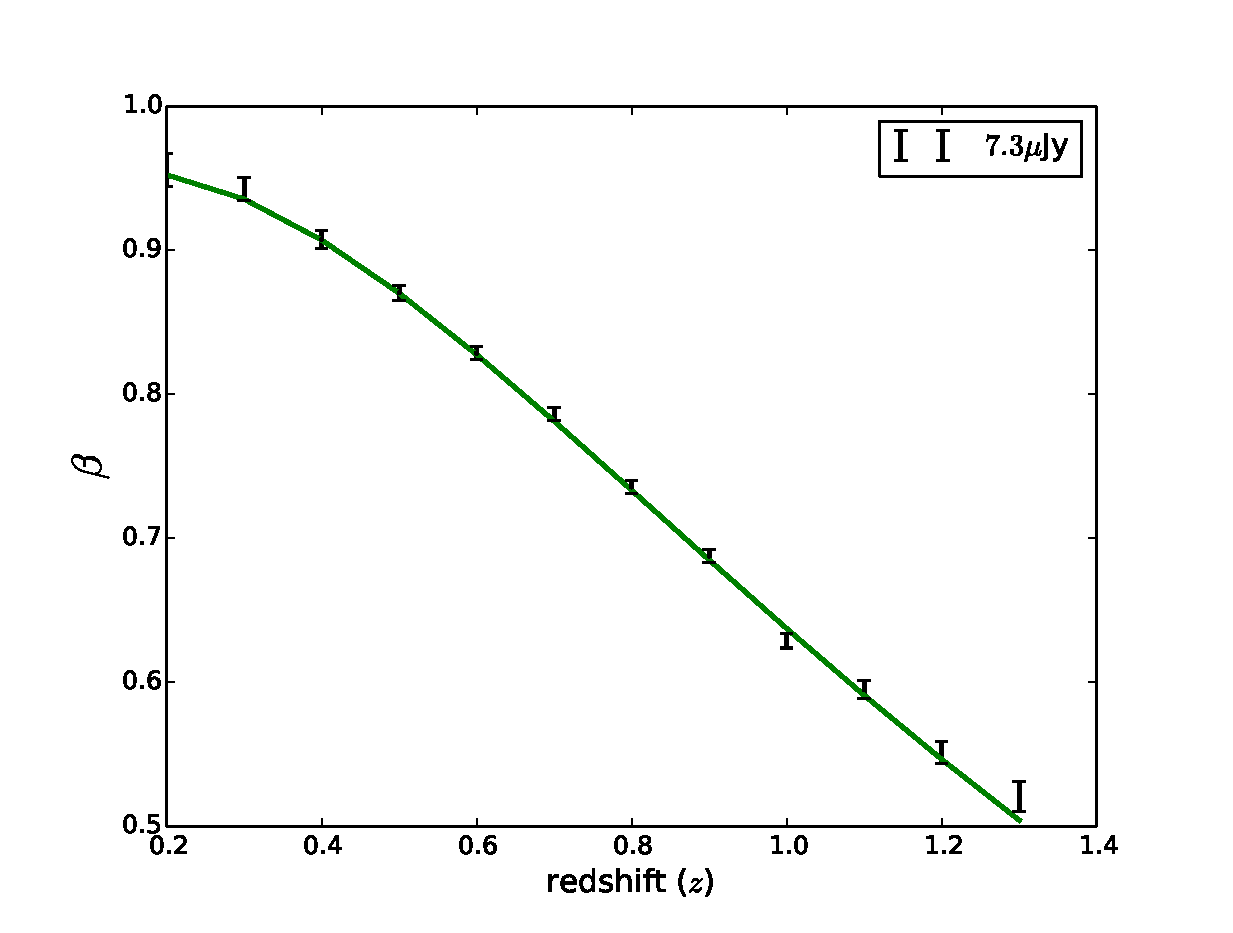
\includegraphics[height=7cm,width=9cm]{plots/beta_errs_7point3mJy_modified_diff_14bins.eps}
\caption{Simulated data points using the errors on Fig.~\ref{fig:fraction} for SKA2 ( $S_{\rm rms} = 7.3 \mu $Jy ): $D_A(z)$ (top), $H(z)$ (middle) and $\beta(z)$ (bottom).}
\label{fig:H_z_D_a_f}
\end{figure}
\end{center}


%###################################
\subsection{ Wiggles-only method}
%###################################


For forecasting based on the BAO, we can use a simplified approach, that has been called the wiggles-only method \citep{Seo:2007ns}.  The power spectrum in this approach is of the form
$ P_b \propto {\sin (ks)}/{ks}$.
The BAO scale is sufficiently large-scale that it is little affected by non-linear matter clustering, non-linear galaxy bias and non-linear redshift distortions. 
However, the BAO peak is damped and widened by non-linear effects, which can be modelled via non-linearity parameters $k_{\rm S}$, $\Sigma_{\perp}$ and $\Sigma_{\|}$: 
\begin{eqnarray}
 P_{ b} &=& \sqrt{8\pi^2} A_0 P_{0.2}\frac{\sin{ks}}{ks} \label{eq:gausilk} \\ \nonumber
 &&\times \exp{\left[-\left({k\over k_{\rm S}}\right)^{1.4}-{k^2 \over 2} \left\{(1-\mu^2)\Sigma_\perp^2+\mu^2\Sigma_\parallel^2\right\} \right]},  
 \end{eqnarray}
where
\begin{eqnarray}
k_{\rm S} = 1.6(\Omega_b h^2)^{0.52}(\Omega_{{\rm cdm}} h^2)^{0.73}\left[1+(10.4\Omega_{{\rm cdm}} h^2)^{-0.95}\right],
\end{eqnarray}
and
\begin{eqnarray}
 \Sigma_\perp=\Sigma_0 D, \quad   \Sigma_\parallel=\Sigma_0 (1+f)D.
\end{eqnarray}
Here  $A_0 = 0.5817$ is a normalization factor and $P_{0.2}(z)$ is galaxy power at $k=0.2h{\rm\;Mpc^{-1}}$ and redshift $z$.
 $\Sigma_\perp$ is the r.m.s. displacement across and $\Sigma_\parallel$ is the r.m.s. displacement  along the line of sight, and
$\Sigma_0 =12.4h^{-1}\,$Mpc for a cosmology with $\sigma_8=0.9$.
 
If we assume that $s$ is well measured from CMB observations, then the errors on $s_\perp$ and $s_\|$  are virtually equivalent to the errors on $D_A(z)$ and $H(z)$. 
We follow  \cite{Seo:2007ns} and choose
\begin{equation}
 \theta_1=\ln{s_\perp^{-1}}, \quad \theta_2=\ln{s_\parallel}.
 \end{equation}
 Then  the Fisher matrix  evaluated around the fiducial cosmology with  $s_\perp=s_\parallel=s$, is given by:
\begin{eqnarray}\label{FIJ_DEV}
F_{ij}&=&\int_{-1}^{1}d\mu\int_{0}^{\infty}k^2dk \frac{V_{\rm survey}}{\left[P^z+n^{-1}\right]^2}\nonumber \\
& \times & \left[ A_0 P_{0.2}  R\frac{\partial P_{b}}{\partial \ln (ks)} \right ]^2 
 \frac{\partial \ln (ks)}{\partial \theta_i}\frac{\partial \ln (ks)}{\partial \theta_j} .
\end{eqnarray}


\subsection{Constraints on the BAO}
The measurements of the BAO scale are constrained by  two types of errors,  cosmic variance and  shot noise. Shot noise reflects the limits on reconstructing the matter distribution from galaxy surveys,  and  is  inversely proportional to the number of galaxies at a given survey volume. Upcoming surveys such as the SKA will limit shot noise. 


Cosmic variance which is the uncertainty that results from observing only part of the universe at a specific time,  limits our statistical knowledge on a cosmological scale. Shot noise and cosmic variance are equal when $n P_{0.2} = 1$.

\cite{Abdalla:2009wr} predict that the  full SKA2 survey, up  to $z \sim 1.4$, will be dominated  by cosmic variance.  Fig.~\ref{fig:cosmic_variance} shows that  cosmic variance is dominant  up to $z\sim 1.8$ and the effect of the bias is clear.


\section{Results}
Our work considers the SKA, and looks at the  Euclid galaxy redshift  survey  for comparison. 
\subsubsection{SKA}\label{SKA}
When we forecast for the SKA1, we consider different possibilities of  $S_{\rm rms}$;
\begin{itemize}
\item[-] 70$\mu $Jy as the best case scenario,
\item[-] 100$\mu $Jy as a realistic case  , 
\item[-]  and 200$\mu$Jy  as a pessimistic case. 
\end{itemize}
The sky coverage area for SKA1 $\sim$ 5000 deg$^2$, see Table~\ref{tab:surveys}.
Similarly, we forecast  for  SKA2,  with different $S_{\rm rms}$,
\begin{itemize}
\item[-]  3$\mu $Jy as the best case scenario, 
\item[-]  7.3$\mu $Jy as a realistic case,
\item[-]  and 23$\mu $Jy as a pessimistic case.
\end{itemize}
SKA2 will have a sky coverage of $30000\,$deg$^2$, see Table~\ref{tab:surveys}. 



For all cases (SKA1 and SKA2) $k_{\rm max} = 0.5 h\,$Mpc$^{-1}$ and $k_{\rm min}  = 10^{-3}h\,$Mpc$^{-1}$. 

We create redshift bins between $0.01$ and $2.0$, and for each $S_{\rm rms}$ case the maximum redshift limit, $ z_{max}$ is different.  $z_{max}$ is  set by setting the minimum value for $n(z)$ to  $10^{-5} \ h^{3} {\rm Mpc}^{-3}$. Where the redshift bins have  a number density less than this limit it does not improve the estimation of error in the Fisher matrix. Tables~\ref{table:Da_H_0_1_Srms} and \ref{table:Da_H_7point3_23_Srms}  show each case of $S_{\rm rms}$  maximum redshift.

\subsubsection{Euclid}\label{Euclid}
The  Euclid survey is supposed to be a combination between a galaxy survey and a weak lensing survey. To compare the performance of the SKA with other upcoming surveys, we consider the Euclid redshift galaxy survey using the reference  case described in \cite{2013LRR....16....6A}.   

\subsubsection{ 0 Noise case}
We also consider another general case, for all of the cases mentioned above (\ref{Euclid} and \ref{SKA}),  we assume the number density is infinite, $1/n(z) \sim 0$.



%######################################
\subsection{Errors on $D_A$ and $H(z)$}
%#####################################



Using  the $2\times2$ Fisher matrix defined in Eq.~(\ref{FIJ_DEV}), the errors on $\ln{D_A(z)}$ and $\ln{H(z)}$ are computed \citep{Seo:2007ns}:
\begin{equation}
\sigma_{\ln{D_A}}  = \sqrt{(F^{-1})_{11}}, \quad \sigma_{\ln{H}}  =  \sqrt{(F^{-1})_{22}} .
\end{equation}
In the case where the tangential and radial BAO scales are assumed to be equal, the error in  $\ln{R}$ can be computed using \citep{Seo:2007ns}:
\begin{equation}
 \sigma_{\ln R}^2
= \frac{\sigma_{\ln D_A}^2\left(1-r^2\right)}{1+2r\sigma_{\ln
D_A}/\sigma_{\ln H}+\sigma_{\ln D_A}^2/\sigma_{\ln H}^2},
\label{eq:sigmaR2}
\end{equation}
where 
\begin{equation}
r = {F_{12}\over \sqrt{F_{11} F_{22}}}.
\end{equation}





Fig.~\ref{fig:fraction} shows the fractional percentage error on the tangential component ($\sigma_H/H \%$), the radial component ($\sigma_{D_A}/D_A \% $) and the  linear RSD parameter ($\sigma_\beta/ \beta \%$) for both cases SKA1 and SKA2. 

In order to indicate how minimal  the uncertainty for the SKA2 measurements will be, we produced  simulated data points in the given  redshift range using the fractional errors for $S_{\rm rms}= 7.3 \mu$Jy (one of SKA2 cases), the results are shown in Fig.~\ref{fig:H_z_D_a_f}. 


%############################
\subsection{Error propagation to  $\beta$}
%############################

From the uncertainty of $\ln R$ in Eq.~(\ref{eq:sigmaR2}), we can use the propagation of error rule to find the uncertainty of $\beta$, assuming that the error contribution from $\Sigma_z \approx 0$:
\begin{equation}
\sigma_\beta  = \frac{(1+\mu^2 \beta)^{2}}{2 \mu^2} \sigma_{ \ln R(\mu)} .
\end{equation}
The errors in $\beta$  versus redshift for different sensitivities  are shown in Fig.~\ref{fig:fraction}.

%##########################
 \subsection{Error propagation to dark energy equation of state}
%#################################
\label{sec:darkenergy}

We parameterize $w(z)$ via Eq.~(\ref{wz}), and
propagate the errors in $D_A(z)$ and $H(z)$, Eq.~\ref{eq:Fij}, to the cosmological parameters using:
\begin{equation}
\tilde{F}_{\alpha\beta}=\sum_{ij}{\partial \theta_i\over \partial \theta_\alpha}{\partial \theta_j\over \partial \theta_\beta}F_{ij}.
\end{equation}
%Here $\tilde{F}_{\alpha\beta}$ is the Fisher matrix  forecast the cosmological parameters, 
% is the Fisher matrix for $D_A(z)$ and $H(z)$, so that
where $\theta_i=(\ln D_A, \ln H)$ and $\theta_\alpha=(w_0,w_a,\Omega_{\rm cdm}, \Omega_b, \Omega_K, h)$, for detailed calculations see Eq.~\ref{Eq:drv}. 

%##########################
\subsubsection{ Adding priors}
%##########################


Forecasting the errors for  the cosmological parameters $w_0$, $w_a$, $\Omega_{\rm cdm}$, $\Omega_b$, $\Omega_K$ and $h$, is  achieved by adding a diagonal  prior matrix,  derived from Plank's prior matrix \citep{2013LRR....16....6A}, to the SKA Fisher matrix, see Table~\ref{tab:planck_prior}.


\begin{table*}\label{tab:planck_prior}
\begin{tabular}{@{}lc|cccccccc}
\hline \hline
                        - &  $n_s$  &    $ w_0$                &         $ w_a$                &          $   \Omega_b$   &    $ \Omega_K $          &         $ \Omega_{\rm cdm} $    &$ h  $ &   $\sigma_8$  \\ \hline \hline 
              $n_s$    &  1.995792e+05 & -3.736675e+04 & -1.049368e+04   & 1.399776e+06
   & 5.586439e+05 &  1.911997e+06&  -7.651819e+04 & -2.238062e+03    \\
              $  w_0$ & -3.736675e+04 &  1.839286e+05 &  5.165256e+04  & -7.420507e+06
  & -3.987583e+06 & -1.252519e+07  & 1.324383e+06  & -4.515591e+02 \\
                $ w_a$& -1.049368e+04 &  5.165256e+04 &   1.450555e+04  & -2.083896e+06
  &  -1.119830e+06   & -3.517442e+06 &    3.719258e+05 & -1.268110e+02 \\
   $  \Omega_b$ & 1.399776e+06   &-7.420507e+06 &  -2.083896e+06 &  3.649438e+08
   & 1.585996e+08 &  5.661366e+08 &  -5.168785e+07 &  3.203389e+04  \\
     $\Omega_K $&  5.586439e+05  & -3.987583e+06 &  -1.119830e+06 &  1.585996e+08
  &  8.705355e+07 &  2.705270e+08 & -2.917404e+07 &  1.884381e+04 \\
    $ \Omega_{\rm cdm} $ &  1.911997e+06 & -1.252519e+07  & -3.517442e+06   & 5.661366e+08 &  2.705270e+08  & 9.116277e+08 & -8.940715e+07 &  6.346286e+04 \\
                  $  h$ &   -7.651819e+04  & 1.324383e+06 &  3.719258e+05  &-5.168785e+07
  & -2.917404e+07 & -8.940715e+07 &  9.889490e+06  & -1.018381e+04\\
  $\sigma_8$ & -2.238062e+03 & -4.515591e+02 &  -1.268110e+02 &  3.203389e+04
   & 1.884381e+04 &  6.346286e+04  & -1.018381e+04 &  1.517096e+04\\
   \\
\hline
\end{tabular}

\caption{Plank's prior matrix corresponds to the cosmological parameters of interest.}
\end{table*}
We also add prior information about the
angular diameter distance out to $z=1090$  from the last scattering surface (LSS) using Eq.~(\ref{add_lss}):
\begin{equation}
\frac{\sigma_{D_A(1090)}}{D_A(1090)}= 0.001
\end{equation}
Our predictions have been based on three assumptions: 
\begin{itemize}
\item[-] Non-flat universe: When we  estimate the errors for $w_0, w_a, \Omega_{{\rm cdm}}, \Omega_b, \Omega_K, h$, the Fisher matrix  is a $6\times 6$ matrix, see the results in Table~\ref{Table1:summary-wa-w0_all}; The results  for $ S_{\rm rms} = 100 \mu $Jy (SKA1)  and $ S_{\rm rms} = 7.3 \mu $Jy (SKA2) are also shown in Fig.~\ref{Fig:w_wa}.
\item[-] Flat universe: We fixed $\Omega_K=0$, and forecast the errors for $w_0, w_a, \Omega_{{\rm cdm}}, \Omega_b, h$, therefore  the Fisher matrix is a $5 \times 5$ matrix, the results are shown in  Table~\ref{Table:summary_w_wo_ok_fixed_all}.
% Fig.~\ref{Fig:w_wa_two_cases} shows the marginalized errors for $w$ and $w_a$ for the current case and the non-flat case where $ S_{\rm rms} = 7.3 \mu $Jy.
\item[-] We assume a non flat universe and constant $w=-1$,  then Fisher matrix is $5 \times 5$. Table~\ref{Table:summary_w_ok_all}  shows the errors on the cosmological parameters and Fig.~\ref{Fig:w_ok} shows the constraints on $w$ and $\Omega_K$ for $S_{{\rm rms}}= 100 \mu$Jy and $7.3 \mu$Jy.
\end{itemize}
 Note that for all cases  we added Planck priors and the prior information about the angular diameter distance  to the SKA Fisher matrices.


\begin{table*}
\caption{Shows different $S_{\rm rms}$, $\sigma_{D_A}/{D_A} \%$ and $\sigma_{H}/H \%$, and  the corresponding error values of $w_0, \  w_a, \ \Omega_{{\rm cdm}}, \ \Omega_b,\Omega_K,\  h$. Last column shows FoM of the SKA.}
\begin{tabular}{ |l|l|l|l|l|l||l||l|l|l|l|}
\hline
\hline 
\multirow{1}{*}{Setup}& $S_{\rm rms}$  [$\mu$Jy]  & $\sigma_{D_A}/{D_A} \%$ & $\sigma_{H}/H \%$ & $\sigma_{w_0}$ &  $\sigma_{w_a}$ &  $\sigma_{\Omega_{{\rm cdm}}} $ & $\quad \sigma_{\Omega_b}$ & $ \sigma_{\Omega_K} $ & $\sigma_{h}$ & DETF FoM \\
\hline
\multirow{1}{*}{SKA1 (5000 deg$^2$)}
  & 70  & 1.4& 2.82 & 0.5584 & 3.09 & 0.007 & 7.174e-03 & 0.030 & 0.020 & 07  \\
 & 100 & 1.9&3.79 & 1.0636 & 6.06 & 0.015 & 1.467e-02 & 0.062 & 0.041 & 03  \\
  & 200 & 2.9 & 5.75  & 2.1059 & 12.24 & 0.030 & 3.048e-02 & 0.129 & 0.086 & 01  \\
\hline
\hline
\multirow{1}{*}{SKA1 (5000 deg$^2$)}
  & 0 noise &0.13 & 0.31 & 0.0324 & 0.11 & 0.001 & 5.385e-04 & 0.001 & 0.003 & 492  \\
\hline
\multirow{3}{*}{SKA2 (30000 deg$^2$)}
% & 1 &  0.04046 & 0.18854 &  0.00666& 5.197427 $\times 10^{-5}$ & 0.00221  & 0.43911 &378 \\
  & 3 &0.09 & 0.19 & 0.0248 & 0.07 & 0.001 & 5.195e-04 & 0.001 & 0.003 & 910  \\
   &7.3& 0.14 & 0.30 & 0.0362 & 0.12 & 0.001 & 5.773e-04 & 0.001 & 0.003 & 496  \\
  & 23 &0.28 & 0.58 & 0.0727 & 0.32 & 0.001 & 8.699e-04 & 0.003 & 0.004 & 157  \\
  \hline
  \hline
\multirow{1}{*}{SKA2 (30000 deg$^2$)}
 & 0 noise & 0.05& 0.13 & 0.0178 & 0.05 & 0.001 & 4.874e-04 & 0.001 & 0.002 & 1460  \\

  \hline

\multirow{1}{*}{Euclid (15000 deg$^2$)}
 & -  &0.22 & 0.40 & 0.0435 & 0.16 & 0.001 & 5.600e-04 & 0.001 & 0.003 & 327  \\
\hline
\hline
\multirow{1}{*}{Euclid (15000 deg$^2$)}
 & 0 noise  &0.13 &0.29  & 0.0328 & 0.12 & 0.001 & 5.406e-04 & 0.001 & 0.003 & 462  \\
\hline
\end{tabular}
\label{Table1:summary-wa-w0_all}
\end{table*}

 
\begin{table*}
\caption{Shows different values of the $S_{\rm rms}$, and the corresponding  error values  of $w_0, \  w_a, \ \Omega_{{\rm cdm}}, \ \Omega_b, \ h$  where $\Omega_K$ is {\bf fixed}. Last column shows FoM of the SKA.}
\begin{tabular}{ |l|l|l|l||l||l|l|l|l|}
\hline
\hline 
\multirow{1}{*}{Setup}& $S_{\rm rms}$  [$\mu$Jy] & $\sigma_{w_0}$ &  $\sigma_{w_a}$ &  $\sigma_{\Omega_{{\rm cdm}}} $ & $\quad \sigma_{\Omega_b}$ & $\sigma_{h}$ & DETF FoM \\
   \hline
\multirow{2}{*}{SKA1 (5000 deg$^2$) }
   & 70 & 0.1108 & 0.40 & 3.549e-04 & 3.430e-04 & 0.002 & 88  \\
   & 100 & 0.1553 & 0.55 & 3.558e-04 & 3.438e-04 & 0.002 & 63  \\
      & 200 & 0.2612 & 0.93 & 3.585e-04 & 3.467e-04  & 0.002 & 37  \\
\hline
  \hline
\multirow{1}{*}{SKA1 (5000 deg$^2$)}
 & 0 noise & 0.0244 & 0.11 & 2.035e-04 & 2.772e-04  & 0.001 & 828  \\
     \hline
\multirow{3}{*}{SKA2 (30000 deg$^2$)}

% & 1 &  0.03163 & 0.11312 &  0.00421& 5.197425 $\times 10^{-5}$ & 0.37207 &796 \\
  & 3 & 0.0146 & 0.06 & 1.863e-04 & 2.724e-04  & 0.001 & 1762  \\
   &7.3& 0.0178 & 0.09 & 2.290e-04 & 2.895e-04  & 0.001 & 1066  \\ 
     & 23& 0.0253 & 0.12 & 3.103e-04 & 3.235e-04 & 0.002 & 472  \\
      \hline
  \hline
\multirow{1}{*}{SKA2 (30000 deg$^2$)}
 & 0 noise& 0.0118 & 0.05 & 1.647e-04 & 2.634e-04  & 0.001 & 2609  \\
     \hline

\multirow{1}{*}{Euclid (15000 deg$^2$)}
 & -  & 0.0347 & 0.15 & 2.345e-04 & 2.893e-04  & 0.002 & 489  \\
  \hline
          \hline
\multirow{1}{*}{Euclid (15000 deg$^2$)}
 & 0 noise& 0.0268 & 0.12 & 2.002e-04 & 2.757e-04  & 0.001 & 763  \\
     \hline
\end{tabular}
\label{Table:summary_w_wo_ok_fixed_all}
\end{table*}

 %We also forecast the error on $\Omega_K$  assuming $w = -1$,  for SKA1 and SKA2 (see Table~\ref{Table:summary_w_ok_all} and Fig.~\ref{Fig:w_ok}) 
\begin{table*}
\caption{Shows different values of $S_{\rm rms}$ and their corresponding error values of  $w, \Omega_K,  \Omega_{{\rm cdm}}, \Omega_b, h$  for the SKA, on this case we assume  $w=w_0= -1$.}
\begin{tabular}{ |l|l|l|l||l||l|l|l|l|}
\hline
\hline 
\multirow{1}{*}{Setup}& $S_{\rm rms}$ [$\mu$Jy] & $\sigma_{w_0}$ &  $\sigma_{\Omega_K}$ &  $\sigma_{\Omega_{{\rm cdm}}} $ & $\quad \sigma_{\Omega_b}$ & $\sigma_{h}$ \\
 \hline
\multirow{2}{*}{SKA1 (5000 deg$^2$) }

  & 70& 0.0417 & 2.409e-03 & 5.5e-04 & 6.187e-04 & 6.194e-04  \\
   & 100& 0.0492 & 2.835e-03 & 6.1e-04 & 6.948e-04 & 6.212e-04  \\
     & 200& 0.0555 & 3.194e-03 & 6.7e-04 & 7.614e-04 & 6.232e-04  \\
\hline
 \hline
\multirow{1}{*}{SKA1 (5000 deg$^2$)}
 & 0 noise &  0.0058 & 5.424e-04 & 3.4e-04 & 3.743e-04 & 6.152e-04  \\
 \hline
\multirow{3}{*}{SKA2 (30000 deg$^2$)}

% & 1 &  0.01432 & 0.00135 &  0.22799 & 5.568670 $\times 10^{-5} $ & 0.00124  \\
  & 3 & 0.0048 & 4.996e-04 & 3.3e-04 & 3.695e-04 & 6.115e-04  \\
 &7.3& 0.0059 & 5.302e-04 & 3.3e-04 & 3.708e-04 & 6.123e-04  \\
  & 23&0.0104 & 7.087e-04 & 3.4e-04 & 3.826e-04 & 6.135e-04  \\
  \hline
     \hline
\multirow{1}{*}{SKA2 (30000 deg$^2$)}
 & 0 noise & 0.0042 & 4.897e-04 & 3.3e-04 & 3.683e-04 & 6.086e-04  \\
 \hline

\multirow{1}{*}{Euclid (15000 deg$^2$)}
 & - &0.0075 & 6.049e-04 & 3.4e-04 & 3.785e-04 & 6.164e-04  \\
 \hline
    \hline
 \multirow{1}{*}{Euclid (15000 deg$^2$)}
 & 0 noise& 0.0059 & 5.447e-04 & 3.4e-04 & 3.749e-04 & 6.157e-04  \\
 \hline
\end{tabular}
\label{Table:summary_w_ok_all}
\end{table*}

\begin{figure}
\begin{center}
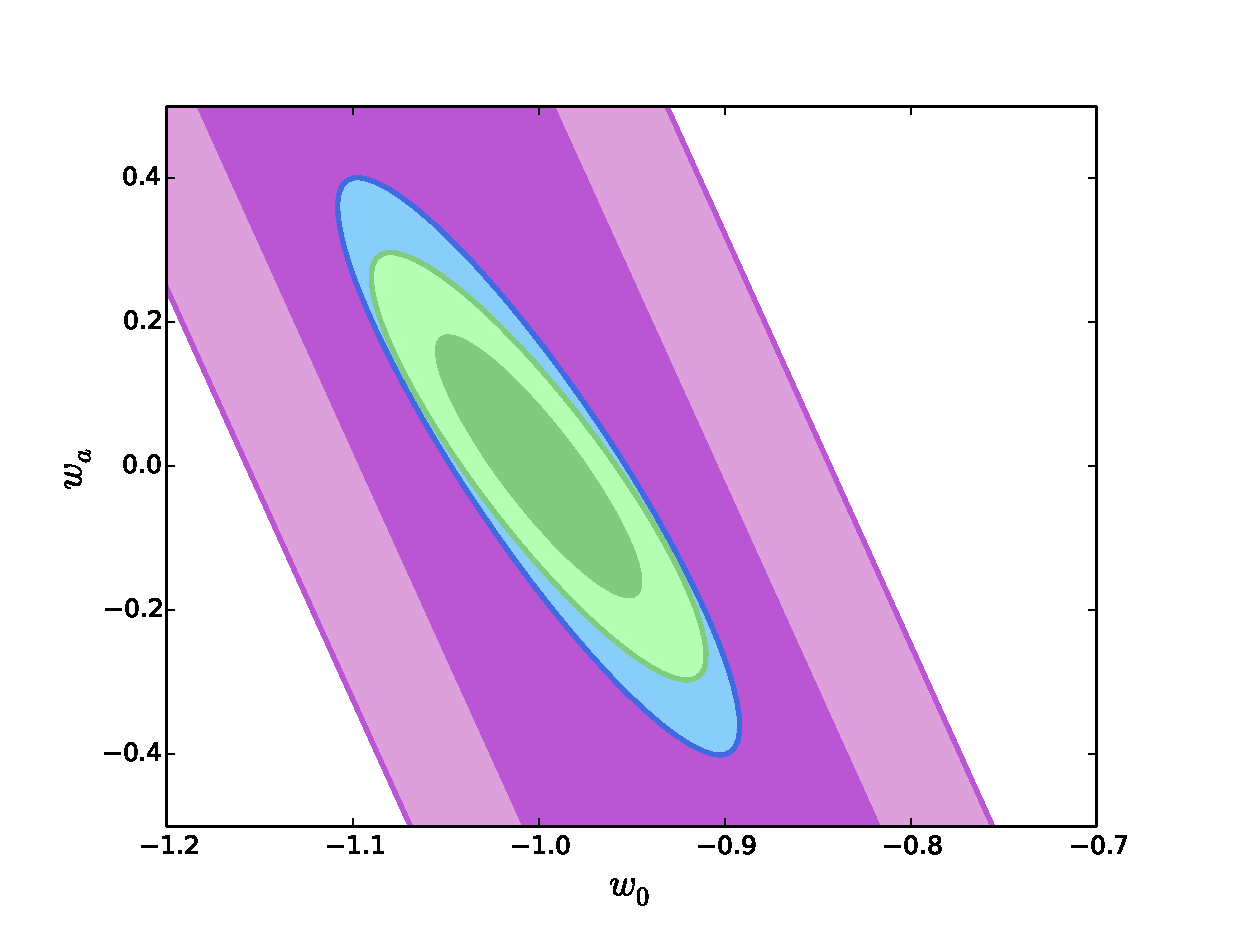
\includegraphics[height=8.0cm,width=9.0cm]{plots/output_ellipse_w0_wa_14bins_70_3.eps} 
\caption{Projected constraints $1 \sigma$ and $2\sigma$ confidence limits on the dark energy parameters $w_0$ and $w_a$ for  SKA1+Planck priors with $S_{\rm rms} = 100 \mu $Jy (purple), SKA2+Planck priors with  $S_{\rm rms} = 7.3 \mu $Jy (green) and Euclid galaxy survey + Planck priors (blue).}
\label{Fig:w_wa}
\end{center}
\end{figure}

%\begin{figure}
%\begin{center}
%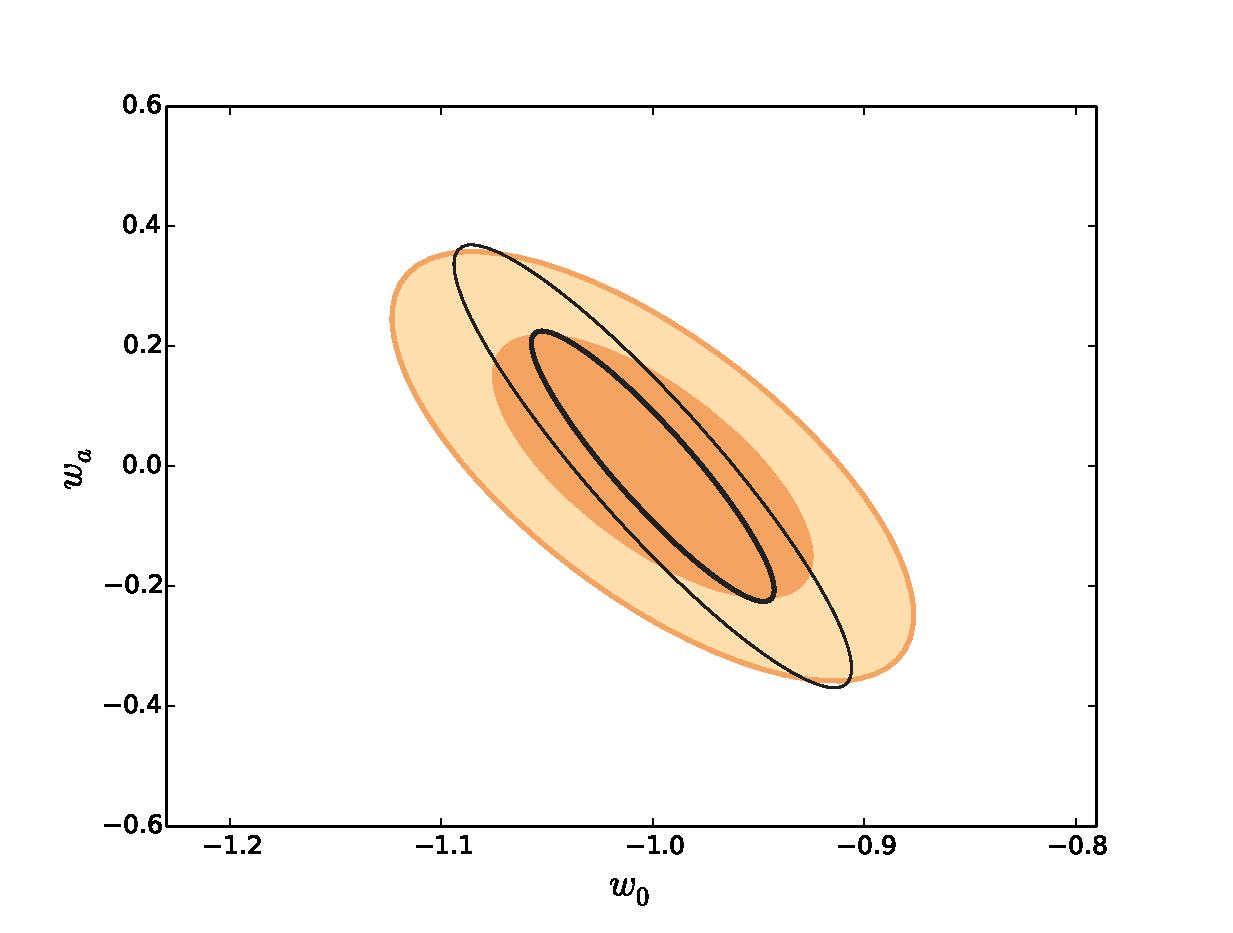
\includegraphics[height=8.0cm,width=9.0cm]{plots/output_ellipse_w0_wa_7point3_muJy_14bins.eps} 
%\caption{Projected constraints on the dark energy parameters $w_0$ and $w_a$ for SKA2+Planck priors when $\Omega_K$ marginalized over (brown). Lines (black) show the $1 \sigma$ and $2\sigma$ confidence limits for the SKA2+Planck priors when $\Omega_k$ is fixed. The results corresponds  to $S_{\rm rms} = 7.3 \mu $Jy. }
%\label{Fig:w_wa_two_cases}
%\end{center}
%\end{figure}



\begin{figure}
\begin{center}
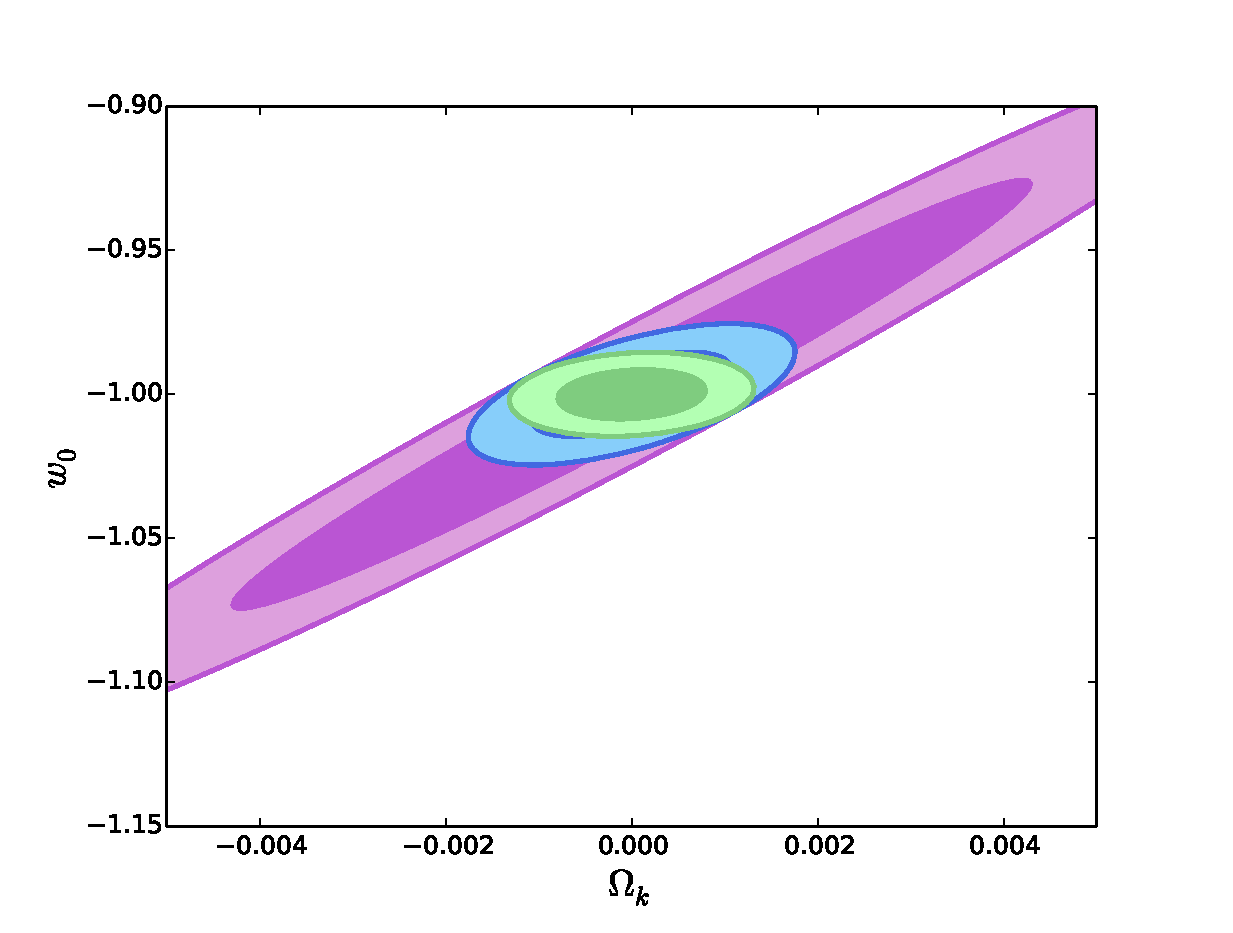
\includegraphics[height=8.0cm,width=9.5cm]{plots/output_ellipse_w0_OK_14bins.eps} 
\caption{Projected constraints on  $w_0$ and $\Omega_K$, $1 \sigma$ and $2\sigma$ confidence limits  for the SKA1+Planck priors where  $S_{\rm rms} = 100 \mu $Jy (red), for the SKA2+Planck priors where  $S_{\rm rms} = 7.3 \mu $Jy (green) and  for Euclid galaxy survey+Plank priors (blue).}
\label{Fig:w_ok}
\end{center}
\end{figure}

%================================
\subsection{Figure of Merit}
%================================
We define the figure of merit (FoM) as
\begin{equation}
{\rm FoM} = \sqrt{{\rm det}( F )},
\end{equation}  
which is also equivalent to the inverse of the $1-\sigma$ ellipse in units of the area of the unit circle \citep{BASSETT2011, Coe:2009xf}.
We used this definition  to find the FoM for the flat case and the non-flat case in Tables~\ref{Table1:summary-wa-w0_all} and \ref{Table:summary_w_wo_ok_fixed_all}. 
%%==================================
%\section{Conclusion}
%%==================================
%Attempting to explore the abilities of different SKA stages. We ran the SAX$^3$ simulation to get simulated $dN/dz$ samples for different $S_{\rm{rms}}$. The galaxy bias also has been estimated. 
%
%In this work we didn't try to match
%the $S_{\rm{rms}}$ from the simulation with the survey specification, although the simulated $S_{\rm{rms}}$  give a sense  of how well each stage and survey will perform with respect to the cosmological parameters.  
%
%We used Wiggles-only forecasting method to estimate the errors on the radial and tangential component of the BAO, then we propagate the errors to the dark energy equation of state parameters (parameterized $w$) and we marginalize over the cosmological parameters affect $w$. We explored different cases with different $S_{\rm{rms}}$. For all cases we force priors on the cosmological parameters using Plank prior matrix, Eq.~(\ref{cov_priors}) and $D_A$ information from LSS.
%
%We forecast the errors on $w_0$ and $w_a$ assuming two cases, non-flat universe (see Table~\ref{Table1:summary-wa-w0_all}, Fig.~\ref{Fig:w_wa}) and a flat universe where $\Omega_K$ is fixed to zero (see Table~\ref{Table:summary_w_wo_ok_fixed_all}). We also consider a case where $w$ is constant and $\Omega_K$ is varying (see Table~\ref{Table:summary_w_ok_all}, Fig.~\ref{Fig:w_ok}).
%
%The accuracy from different SKA stages were explored. We find that for the SKA1 stages, an HI galaxy survey  with area 5000 deg$^2$ doesn't reach a proper accuracy to explore the nature of $w(z)$. For the SKA later stage where the $S_{\rm{rms}}$'s are significantly low, the area will reach 30000 deg$^2$, the results shows that  SKA2 will be a great tool to explore the nature of $w$, see below.
%
%\[
%\begin{array}{c|c|c|c|c}
%\hline
%\\
%& S_{\rm rms}  [ \mu\mbox{Jy}] &  \sigma_{w_0} & \sigma_{w_a} & \sigma_{\Omega_K}  \\
%\hline
%\\
%w_a \ \mbox{is} \  \mbox{Fixed} &\mbox{SKA1}  \ (\sim 100) & 0.11& - & 0.007  \\ 
%&\mbox{SKA2} \ ( \sim 7.3)   &  0.04 &- &   0.003 \\
%\\
% \hline
% \\
% 
%\Omega_k \ \mbox{is} \  \mbox{Fixed} &\mbox{SKA1}  \ (\sim 100) &0.16  &0.66& -  \\ 
%&\mbox{SKA2} \ ( \sim 7.3)& 0.04 & 0.15 &  - \\ 
%\\
% \hline
% \\
%\mbox{Marginalized} \ \mbox{over} \ \mbox{all}&\mbox{SKA1}  \ (\sim 100)& 0.38  &3.0 &0.032 \\ 
%\quad \mbox{parameters}&\mbox{SKA2} \ ( \sim 7.3)  &   0.05 &  0.14&  0.003   \\ \\
%\hline
%\end{array}
%\]
%


\newpage
\[\]
{\bf Acknowledgements:}\\
SY thanks Pedro Ferreira for valuable guidance, and for hospitality during her visit to Oxford University where part of this work was done.
SY, MS, PO and
RM are supported by the South Africa Square Kilometer Array Project and  the South African National Research Foundation. RM acknowledges support from the UK Science \& Technology Facilities Council (grant ST/K0090X/1).
\newpage
\bibliography{Ska_Forecast_draft1.bib}
\bibliographystyle{mn2e}


\newpage

\appendix

\section{Propagation of error calculations}

Partial derivatives of $D_A$ and $H$ with respect to $w_0$ and 
$w_a$ are given by \citep{Shoji:2008xn}
\begin{eqnarray*}\label{Eq:drv}
{\partial \ln{D_A} \over \partial w_0}
&=&-{3\over2}\Omega_{\rm de}{\int_0^z \ln(1+z^{\prime}) \mathcal{F}(z^{\prime})E(z^{\prime})^{-3}dz^{\prime}
\over\int_0^z E(z^{\prime})^{-1}dz^{\prime}},\\
{\partial \ln{D_A} \over \partial w_a}&=&-{3\over2}\Omega_{\rm de}\nonumber\\
&\times&{\int_0^z  \left\{ \ln(1+z^{\prime})-\frac{z^{\prime}}{(1+z^{\prime})} \right\}\mathcal{F}(z^{\prime})E(z^{\prime})^{-3}dz^{\prime}\over\int_0^z E(z^{\prime})^{-1}dz^{\prime}}, \\
{\partial \ln{D_A} \over \partial  \Omega_{{\rm cdm}}}&=&-{1\over2}{\int_0^z \left\{  (1+ z^\prime)^3 - \mathcal{F}(z^\prime)\right\}  E(z^{\prime})^{-3}dz^{\prime}
\over\int_0^z E(z^{\prime})^{-1}dz^{\prime}},\\
{\partial \ln{D_A} \over \partial \Omega_b}&=&-{1\over2}{\int_0^z\left\{ (1+ z^\prime)^3 - \mathcal{F}(z^\prime)\right\}  E(z^{\prime})^{-3}dz^{\prime} \over\int_0^z E(z^{\prime})^{-1}dz^{\prime}},\\
{\partial \ln{D_A} \over \partial  \Omega_K}&=&-{1 \over2} {\int_0^z\left\{(1+z^{\prime})^2 - \mathcal{F}(z^\prime)\right\}E(z^{\prime})^{-3} \over \int_0^z E(z^{\prime})^{-1}dz^{\prime}}\\\nonumber &+&  \frac{1}{6}  \left(  \int_0^z E(z^{\prime})^{-1}dz^{\prime} \right)^2,\\
{\partial \ln{D_A} \over \partial h}&=& 1 \over h\\
{\partial \ln{H} \over \partial w_0}&=&{3\over2}\Omega_{\rm de} \ln(1+z){\mathcal{F}(z)\over E^2(z)},\\
{\partial \ln{H} \over \partial w_a}&=&{3\over2}\Omega_{\rm de}
\left\{\ln(1+z)-\frac{z}{(1+z)}\right\}{\mathcal{F}(z)\over g(z)},\\
{\partial \ln{H} \over \partial  \Omega_{{\rm cdm}}}&=&{1\over2}\left\{(1+z)^3  - \mathcal{F}(z) \right\}{1\over E^2(z)}, \\
{\partial \ln{H} \over \partial  \Omega_b}&=&{1\over2}\left\{ (1+z)^3  - \mathcal{F}(z) \right\}{1\over E^2(z)}, \\
{\partial \ln{H} \over \partial  \Omega_K}&=& {1\over2}\left\{ (1+z)^2 - \mathcal{F}(z) \right\}{1\over E^2(z)},\\
{\partial \ln{H} \over \partial h}&=& -\frac{1}{h},
\end{eqnarray*}
where $\mathcal{F}(z)$ and $E(z)$ are given by Eq.~(\ref{Fz}) and (\ref{EzandDz}) respectively.

We marginalize over $H_0$, $\Omega_{{\rm cdm}}$, $\Omega_b$ and $\Omega_K$, and we add the distance information from LSS  as
\begin{equation}
F^{total}_{\alpha\beta}(z)=F^{LSS}_{\alpha\beta}
+F^{gal}_{\alpha\beta}(z),
\end{equation}
where we add the
angular diameter distance at $z=1090$ using
\begin{equation}\label{add_lss}
 F^{LSS}_{\alpha\beta} = 10^4 \frac{\partial \ln
  D_A(z=1090)}{\partial q_\alpha}\frac{\partial \ln D_A(z=1090)}{\partial q_\beta}.
\end{equation}


\section{Further Details}
In the section we show the uncertainty on the values of $H$ and $D_A$ at different redshift bins considering different SKA setups (see Table~\ref{table:Da_H_0_1_Srms}, \ref{table:Da_H_7point3_23_Srms} and  \ref{Da_H_200_100_Srms}). Also, the tables show the number of galaxies at each redshift bin.
\begin{table*}
\begin{center}
%\caption{The errors on $D_A$ and $H$ (3rd and 4th column) at different redshift bins for an experiment with  (see Fig.~\ref{fig:H_z_D_a_f}) using survey area 30000 deg$^2$, column 5 and 6 show $\sigma_{D_A}/D_A$ and  $\sigma_H/H$ (see Fig.~\ref{fig:fraction}) at different redshift bins for an experiment with $S_{\rm rms} = 0 \mu$Jy, $ 1 \mu$Jy and $ 3 \mu$Jy. The 7th column shows the number of galaxies, where the last column show the survey volume.} 
\caption{1st column shows $S_{\rm rms}$ (survey area), where the 2nd column shows the redshift bins. The errors on $D_A$ and $H$ (3rd and 4th column) at different redshift bins. 5th and 6th columns show the percentage error on $D_A$ and $H(z)$ respectively (see Fig.~\ref{fig:fraction}).} %7th column shows the number density of galaxies in each redsift bin. Last column shows the survey volume, Eq.~\ref{Vsurvey}.}
\begin{tabular}{l|l|l|l|l|lc||r}
\hline
\hline 
\multirow{1}{*}{ $S_{\rm rms}$ (Jy) }& z & $\sigma_{D_A} $ [${\rm Mpc}$]&  $\sigma_{H}$ [${\rm Mpc}$] & $\sigma_{D_A}/{D_A} \%$ & $\sigma_{H}/H \%$ &n(z) [$h^{3} {\rm Mpc}^{-3}$] \\
%& $V_{\rm survey}$ [$h^{-3} {\rm Gpc}^3$] \\
\hline
\multirow{20}{*}{3 $\mu$Jy (30000 deg$^2$)}
& 0.02 &  31.70 & 68.79 & 39.51 & 93.55 & 1.14e-01 \\
& 0.04 &  31.75 & 35.75 & 20.25 & 48.25 & 1.35e-01 \\
& 0.06 &  31.08 & 24.20 & 13.52 & 32.41 & 1.42e-01 \\
& 0.08 &  30.35 & 18.36 & 10.12 & 24.40 & 1.44e-01 \\
& 0.1 &  8.30 & 4.16 & 2.27 & 5.49 & 1.42e-01 \\
& 0.2 &  8.11 & 2.41 & 1.23 & 3.05 & 1.13e-01 \\
& 0.3 &  7.40 & 1.73 & 0.83 & 2.08 & 8.11e-02 \\
& 0.4 &  6.74 & 1.37 & 0.62 & 1.58 & 5.58e-02 \\
& 0.5 &  6.18 & 1.17 & 0.50 & 1.28 & 3.76e-02 \\
& 0.6 &  5.72 & 1.03 & 0.42 & 1.07 & 2.50e-02 \\
& 0.7 &  5.35 & 0.94 & 0.37 & 0.93 & 1.65e-02 \\
& 0.8 &  5.06 & 0.88 & 0.33 & 0.82 & 1.08e-02 \\
& 0.9 &  4.86 & 0.84 & 0.30 & 0.74 & 6.99e-03 \\
& 1.0 &  4.74 & 0.82 & 0.29 & 0.68 & 4.52e-03 \\
& 1.1 &  4.72 & 0.81 & 0.28 & 0.64 & 2.90e-03 \\
& 1.2 &  4.81 & 0.82 & 0.28 & 0.62 & 1.86e-03 \\
& 1.3 &  5.03 & 0.85 & 0.29 & 0.61 & 1.18e-03 \\
& 1.4 &  5.42 & 0.91 & 0.31 & 0.61 & 7.50e-04 \\
& 1.5 &  6.05 & 1.00 & 0.34 & 0.64 & 4.70e-04 \\
& 1.6 &  6.98 & 1.14 & 0.40 & 0.70 & 3.00e-04 \\
& 1.7 &  8.34 & 1.35 & 0.47 & 0.79 & 1.90e-04 \\
& 1.8 &  10.30 & 1.67 & 0.58 & 0.93 & 1.20e-04 \\
& 1.9 &  13.15 & 2.15 & 0.75 & 1.15 & 7.00e-05 \\
& 2.0 &  17.29 & 2.88 & 0.99 & 1.47 & 5.00e-05 \\
\hline
\multirow{10}{*}{ 7.3 $\mu$Jy  (30000 deg$^2$) } 
& 0.02 &  31.65 & 68.74 & 39.45 & 93.48 & 2.03e-01 \\
& 0.04 &  31.73 & 35.73 & 20.23 & 48.23 & 1.95e-01 \\
& 0.06 &  31.08 & 24.19 & 13.52 & 32.41 & 1.81e-01 \\
& 0.08 &  30.36 & 18.36 & 10.13 & 24.40 & 1.65e-01 \\
& 0.1 &  8.31 & 4.17 & 2.27 & 5.49 & 1.50e-01 \\
& 0.2 &  8.13 & 2.41 & 1.24 & 3.05 & 8.64e-02 \\
& 0.3 &  7.45 & 1.73 & 0.83 & 2.09 & 4.82e-02 \\
& 0.4 &  6.84 & 1.38 & 0.63 & 1.59 & 2.66e-02 \\
& 0.5 &  6.35 & 1.18 & 0.52 & 1.29 & 1.46e-02 \\
& 0.6 &  6.02 & 1.05 & 0.44 & 1.09 & 7.96e-03 \\
& 0.7 &  5.84 & 0.98 & 0.40 & 0.96 & 4.34e-03 \\
& 0.8 &  5.86 & 0.94 & 0.38 & 0.88 & 2.36e-03 \\
& 0.9 &  6.13 & 0.94 & 0.38 & 0.83 & 1.28e-03 \\
& 1.0 &  6.75 & 0.99 & 0.41 & 0.83 & 6.90e-04 \\
& 1.1 &  7.85 & 1.10 & 0.47 & 0.87 & 3.70e-04 \\
& 1.2 &  9.68 & 1.30 & 0.57 & 0.98 & 2.00e-04 \\
& 1.3 &  12.66 & 1.65 & 0.73 & 1.18 & 1.10e-04 \\
& 1.4 &  17.46 & 2.25 & 1.00 & 1.52 & 6.00e-05 \\
& 1.5 &  25.25 & 3.26 & 1.44 & 2.10 & 3.00e-05 \\
& 1.6 &  37.98 & 4.99 & 2.16 & 3.07 & 2.00e-05 \\
& 1.7 &  58.92 & 8.02 & 3.34 & 4.69 & 1.00e-05 \\
\hline
\end{tabular}
\label{table:Da_H_0_1_Srms}
\end{center}
\end{table*}

\begin{table*}
\caption{This table is a continuation of Table~\ref{table:Da_H_0_1_Srms}}
\begin{tabular}{l|l|l|l|l|lc||r}
\hline
\hline 
\multirow{1}{*}{ $S_{\rm rms}$ (Jy) }& z & $\sigma_{D_A}$ [${\rm Mpc}$]&  $\sigma_{H}$ [${\rm Mpc}$]& $\sigma_{D_A}/{D_A} \%$ & $\sigma_{H}/H\%$ &n(z) [$h^{3} {\rm Mpc}^{-3}$]& $V_{\rm survey}$ [$h^{-3} {\rm Gpc}^3$]\\
\hline
\hline
\multirow{6}{*}{ 23 $\mu$Jy   (30000 deg$^2$)}
& 0.02 &  31.56 & 68.66 & 39.33 & 93.37 & 5.58e-01 \\
& 0.04 &  31.66 & 35.71 & 20.19 & 48.20 & 3.20e-01 \\
& 0.06 &  31.04 & 24.18 & 13.50 & 32.39 & 2.16e-01 \\
& 0.08 &  30.34 & 18.36 & 10.12 & 24.40 & 1.56e-01 \\
& 0.1 &  8.31 & 4.17 & 2.27 & 5.49 & 1.17e-01 \\
& 0.2 &  8.21 & 2.42 & 1.25 & 3.06 & 3.49e-02 \\
& 0.3 &  7.70 & 1.75 & 0.86 & 2.12 & 1.24e-02 \\
& 0.4 &  7.44 & 1.43 & 0.69 & 1.65 & 4.72e-03 \\
& 0.5 &  7.67 & 1.29 & 0.62 & 1.41 & 1.87e-03 \\
& 0.6 &  8.70 & 1.27 & 0.64 & 1.32 & 7.60e-04 \\
& 0.7 &  11.08 & 1.42 & 0.76 & 1.39 & 3.10e-04 \\
& 0.8 &  15.92 & 1.80 & 1.04 & 1.68 & 1.30e-04 \\
& 0.9 &  25.49 & 2.64 & 1.60 & 2.33 & 6.00e-05 \\
& 1.0 &  44.58 & 4.40 & 2.71 & 3.68 & 2.00e-05 \\
& 1.1 &  82.97 & 8.13 & 4.93 & 6.45 & 1.00e-05 \\
\hline
\multirow{3}{*}{ 70 $\mu$Jy (5000 deg$^2$) }
& 0.02 &  77.27 & 168.16 & 96.30 & 228.68 & 7.22e-01 \\
& 0.04 &  77.54 & 87.46 & 49.45 & 118.05 & 3.06e-01 \\
& 0.06 &  76.06 & 59.24 & 33.08 & 79.36 & 1.67e-01 \\
& 0.08 &  74.43 & 45.00 & 24.83 & 59.81 & 1.02e-01 \\
& 0.1 &  20.43 & 10.22 & 5.58 & 13.47 & 6.55e-02 \\
& 0.2 &  20.76 & 6.02 & 3.15 & 7.61 & 1.06e-02 \\
& 0.3 &  21.90 & 4.61 & 2.45 & 5.56 & 2.21e-03 \\
& 0.4 &  28.86 & 4.49 & 2.67 & 5.17 & 5.10e-04 \\
& 0.5 &  51.80 & 6.02 & 4.20 & 6.58 & 1.30e-04 \\
& 0.6 &  122.61 & 11.49 & 9.04 & 11.93 & 3.00e-05 \\
& 0.7 &  346.23 & 29.29 & 23.80 & 28.81 & 1.00e-05 \\
 \hline\\\\
\end{tabular}
\label{table:Da_H_7point3_23_Srms}
\end{table*}



\begin{table*}
\caption{This table is a continuation of Table~\ref{table:Da_H_7point3_23_Srms}}
\begin{tabular}{l|l|l|l|l|lc||r}
\hline
\hline 
\multirow{1}{*}{ $S_{\rm rms}$ (Jy) }& z & $\sigma_{D_A}$ [${\rm Mpc}$]&  $\sigma_{H}$ [${\rm Mpc}$]& $\sigma_{D_A}/{D_A} \%$ & $\sigma_{H}/H\%$ &n(z) [$h^{3} {\rm Mpc}^{-3}$]& $V_{\rm survey}$ [$h^{-3} {\rm Gpc}^3$]\\
\hline
\hline
\multirow{1}{*}{100 $\mu$Jy (5000 deg$^2$) }
& 0.02 &  77.41 & 168.30 & 96.49 & 228.87 & 2.20e-01 \\
& 0.04 &  77.81 & 87.59 & 49.62 & 118.22 & 1.09e-01 \\
& 0.06 &  76.49 & 59.39 & 33.27 & 79.55 & 6.40e-02 \\
& 0.08 &  75.06 & 45.17 & 25.04 & 60.03 & 4.03e-02 \\
& 0.1 &  20.69 & 10.28 & 5.65 & 13.55 & 2.63e-02 \\
& 0.2 &  22.22 & 6.21 & 3.37 & 7.85 & 4.07e-03 \\
& 0.3 &  28.08 & 5.26 & 3.14 & 6.35 & 7.50e-04 \\
& 0.4 &  52.23 & 6.67 & 4.83 & 7.67 & 1.50e-04 \\
& 0.5 &  142.85 & 13.70 & 11.58 & 14.97 & 3.00e-05 \\
& 0.6 &  495.58 & 41.52 & 36.55 & 43.08 & 1.00e-05 \\
\hline
\multirow{1}{*}{200 $\mu$Jy (5000 deg$^2$) }
& 0.02 &  77.42 & 168.30 & 96.50 & 228.88 & 2.11e-01 \\
& 0.04 &  77.98 & 87.67 & 49.73 & 118.33 & 7.77e-02 \\
& 0.06 &  76.97 & 59.55 & 33.48 & 79.76 & 3.78e-02 \\
& 0.08 &  76.07 & 45.43 & 25.38 & 60.38 & 2.05e-02 \\
& 0.1 &  21.21 & 10.39 & 5.79 & 13.70 & 1.19e-02 \\
& 0.2 &  27.67 & 6.93 & 4.20 & 8.75 & 1.16e-03 \\
& 0.3 &  59.47 & 8.54 & 6.66 & 10.31 & 1.50e-04 \\
& 0.4 &  221.75 & 21.61 & 20.50 & 24.85 & 2.00e-05 \\
\hline\\\\
\end{tabular}
\label{Da_H_200_100_Srms}
\end{table*}


%\bsp

\label{lastpage}

\end{document}
